\documentclass[11pt,a4paper]{article}

% Codificação e idioma
\usepackage[utf8]{inputenc}
\usepackage[T1]{fontenc}
\usepackage[brazil]{babel}

% Fonte: para usar fonte sem serifa como padrão
\usepackage{helvet}
\renewcommand{\familydefault}{\sfdefault}

% Margens de 2cm em todos os lados
\usepackage[a4paper, margin=2cm]{geometry}

% Espaçamento 1,5 entre linhas
\usepackage{setspace}
\onehalfspacing

% Configuração para quebras de linha naturais
\usepackage{parskip}
\setlength{\parskip}{0.3\baselineskip}
\setlength{\parindent}{0pt}

% Pacotes para gráficos, tabelas e links (se necessário)
\usepackage{graphicx}
\usepackage{float}
\usepackage{amsmath,amssymb}
\usepackage{hyperref}
\usepackage{subcaption}
\hypersetup{
    colorlinks=true,
    linkcolor=blue,
    urlcolor=blue
}

% Informações do título e autores
\title{Do meio à arte, da arte ao meio: \\Como o território influencia a criação artística e o tempo define o destaque. Uma análise exploratória das pinturas e esculturas do Metropolitan Museum of Art (MET).}
\author{
  Beatriz Reis Repette \\
  Diego Martins Meditsch \\
  Pedro Henrique Gimenez \\
  Tom Pereira Hunt \\
  \\
  Universidade Federal de Santa Catarina \\
  Florianópolis, 2025
}
\date{}

\begin{document}

\maketitle

% Seção: Introdução e Objetivos
\section{Introdução e Objetivos}
Este trabalho visa reunir, comparar e analisar dados relacionados às obras do Metropolitan Museum of Art (MET), com especial enfoque aos materiais, categorias, culturas e temáticas abordadas. Outro importante paralelo que faremos é com a popularidade das peças em relação às suas características, usando como base uma variável estatística relacionada disponibilizada.
Os dados foram obtidos por meio de uma iniciativa do próprio museu, que disponibiliza os dados do seu acervo publicamente. Os dados foram acessados em 12 de março de 2025 no GitHub, onde foram disponibilizados gratuitamente pelo próprio museu e atualizados pela última vez no dia 17 de junho de 2023 \cite{metOpenAccess}.
A partir da apresentação dos dados coletados, buscamos validar duas principais hipóteses:
\begin{enumerate}
    \item As tendências de materiais na construção artística dentro de uma determinada cultura estão amplamente atreladas à disponibilidade dos materiais na região ocupada pelos povos que se identificam com essa cultura.
    \item A popularidade das obras relaciona-se ao momento socioeconômico cultural das exposições, sendo que as obras destacadas em certo momento capturam essas tendências quanto à temática, tamanho e época de criação das obras;
\end{enumerate}
	Sendo a arte intrinsecamente ligada à cultura de cada época e uma ferramenta irrenunciável de análise histórica, buscamos nesta análise exploratória traçar paralelos quanto à apreciação da arte e à contemporaneidade. Além disso, buscamos encontrar relações entre a construção dessa cultura e a região de onde veio, mostrando que a cultura é construída pelo homem, mas moldada também pelo seu contexto físico, além do político e social.

"A arte é a expressão da sociedade no seu conjunto: crenças, ideias que faz de si e do mundo. Diz tanto quanto os textos do seu tempo, às vezes até mais." --- Georges Duby.

% Seção: Materiais e Métodos
\section{Materiais e Métodos}
Optamos por analisar somente pinturas e esculturas dentre todas as obras do museu, de forma a refinar os recortes a serem feitos, visto que, de modo geral, existe um grande número de obras com origens e características mais específicas, o que tornaria nossa análise menos pertinente para as hipóteses propostas. Assim, não faria sentido analisar a porcentagem de país de origem das obras, por exemplo, se uma grande parte delas fosse "fragmentos de vasos gregos", ou analisar o material de obras quando muitas delas são jornais --- que, apesar de não enviesarem os dados, fariam com que eles perdessem o sentido para as análises que queremos trazer.

Dessa forma, nossa escolha de pinturas e esculturas visa generalizar as análises de região, época, cultura e material, tornando esses dados relevantes para discussão.

Ademais, é importante destacar quais eram as exposições em cartaz na data de atualização dos dados, de forma a garantir a transparência da nossa análise e minimizar vieses.

Mesmo que nem todas elas pareçam influenciar nossa amostra restringida a pinturas e esculturas, por precaução, decidimos listá-las. Abaixo, segue a lista de títulos das exposições, sendo o primeiro nome traduzido e o original em itálico entre parênteses.

\begin{itemize}
    \item Esplendor Samurai: Adornos de Espada do Japão Edo (\textit{Samurai Splendor: Sword Fittings from Edo Japan});
    \item Os Ciprestes de Van Gogh (\textit{Van Gogh's Cypresses});
    \item Karl Lagerfeld: Uma Linha de Beleza (\textit{Karl Lagerfeld: A Line of Beauty});
    \item Arte P.S. 2023: Celebrando o Espírito Criativo das Crianças da Cidade de Nova York (\textit{P.S. Art 2023: Celebrating the Creative Spirit of New York City Kids});
    \item Ganesha: Senhor dos Novos Começos (\textit{Ganesha: Lord of New Beginnings});
    \item Philip Guston: Que Tipo de Homem Eu Sou? (\textit{Philip Guston: What Kind of Man Am I?});
    \item O Álbum de Nova York de Berenice Abbott, 1929 (\textit{Berenice Abbott's New York Album, 1929}).
\end{itemize}

Em relação às variáveis escolhidas, seus nomes no banco de dados (entre parênteses, em itálico), suas classificações, descrições, motivo de escolha e possíveis observações, segue:

\subsection*{Cultura (\textit{Culture})}
\begin{itemize}
    \item \textbf{Classificação:} Variável qualitativa
    \item \textbf{Descrição:} Descreve a qual cultura a obra está relacionada, de acordo com o próprio MET.
    \item \textbf{Motivo de escolha:} Essa é a variável central de nossa análise, embasando e conectando nossas duas hipóteses.
\end{itemize}

\subsection*{Ano do objeto (\textit{Object Begin Date})}
\begin{itemize}
    \item \textbf{Classificação:} Variável quantitativa.
    \item \textbf{Descrição:} Ano de criação do objeto, ou aproximado se não houver registro exato. Extraído diretamente do banco de dados (não foi nossa aproximação).
    \item \textbf{Motivo de escolha:} Esse dado contribuirá para a validação da hipótese 2.
\end{itemize}

\subsection*{Dimensões (\textit{Dimensions})}
\begin{itemize}
    \item \textbf{Classificação:} Variável quantitativa.
    \item \textbf{Descrição:} Não consta no banco de dados original como número único, mas como dimensões (multiplicamos as 2 dimensões para pinturas, resultando em cm², e as 3 dimensões para esculturas, resultando em cm³).
    \item \textbf{Motivo de escolha:}  Esse dado contribuirá para a validação da hipótese 2.
    \item \textbf{Observação:} Separamos pinturas e esculturas para não misturar medidas de volume com medidas de área, o que tiraria o sentido dos dados e impossibilitaria comparação/análise.
\end{itemize}

\subsection*{Meio/Material (\textit{Medium})}
\begin{itemize}
    \item \textbf{Classificação:} Variável qualitativa.
    \item \textbf{Descrição:} Descreve os materiais que compõem a obra, tanto para pinturas quanto para esculturas (exs: óleo sobre tela, mármore).
    \item \textbf{Motivo de escolha:} Esse dado contribuirá para a validação da hipótese 1.
\end{itemize}

\subsection*{Temáticas (\textit{Tags})}
\begin{itemize}
    \item \textbf{Classificação:} Variável qualitativa
    \item \textbf{Descrição:} Palavras que definem a temática da obra, seja de seu contexto, do que representa, de onde vem, etc.
    \item \textbf{Motivo de escolha:} Esse dado contribuirá para a validação da hipótese 2.
    \item \textbf{Observação:} Cada obra pode assumir mais de um valor de tag, mas aqui contamos cada atribuição de tag como uma entrada diferente (uma obra com 2 tags - x e y - conta tanto em número de ocorrências de x quanto de y).
\end{itemize}

\subsection*{É destaque (\textit{IsHighlight})}
\begin{itemize}
    \item \textbf{Classificação:} Variável qualitativa dicotômica.
    \item \textbf{Descrição:} Define se uma obra estava em destaque no momento da coleta dos dados, usado em nossa análise para medir popularidade.
    \item \textbf{Motivo de escolha:} Esse dado contribuirá para a validação da hipótese 2.
\end{itemize}

\subsection*{Variáveis Quantitativas}
As seguintes variáveis quantitativas foram selecionadas para nossa análise:

\begin{itemize}
    \item \textbf{Ano do objeto} (Object Begin Date)
    \item \textbf{Dimensão} (Dimensions) - Separada entre escultura e pintura
    \item \textbf{Ano de entrada no museu} (AccessionYear)
\end{itemize}

\subsection*{Variáveis Qualitativas}
As seguintes variáveis qualitativas foram selecionadas para nossa análise:

\begin{itemize}
    \item \textbf{Cultura} (Culture)
    \item \textbf{Meio/Material} (Medium) - Separado entre escultura e pintura
    \item \textbf{Tags} - Observação: múltiplos valores por objeto
    \item \textbf{Popularidade} (IsHighlight) - \textit{Qualitativa binária}
\end{itemize}

Dada a definição, classificação e descrição das variáveis acima, vamos partir para interpretação dos dados observados.

% Seção: Resultados e Discussões
\section{Resultados e Discussões}

\subsection{A Cultura e o Meio: Investigando a Hipótese 1}
\subsubsection{Panorama Cultural do Acervo}

\begin{figure}[H]
    \centering
    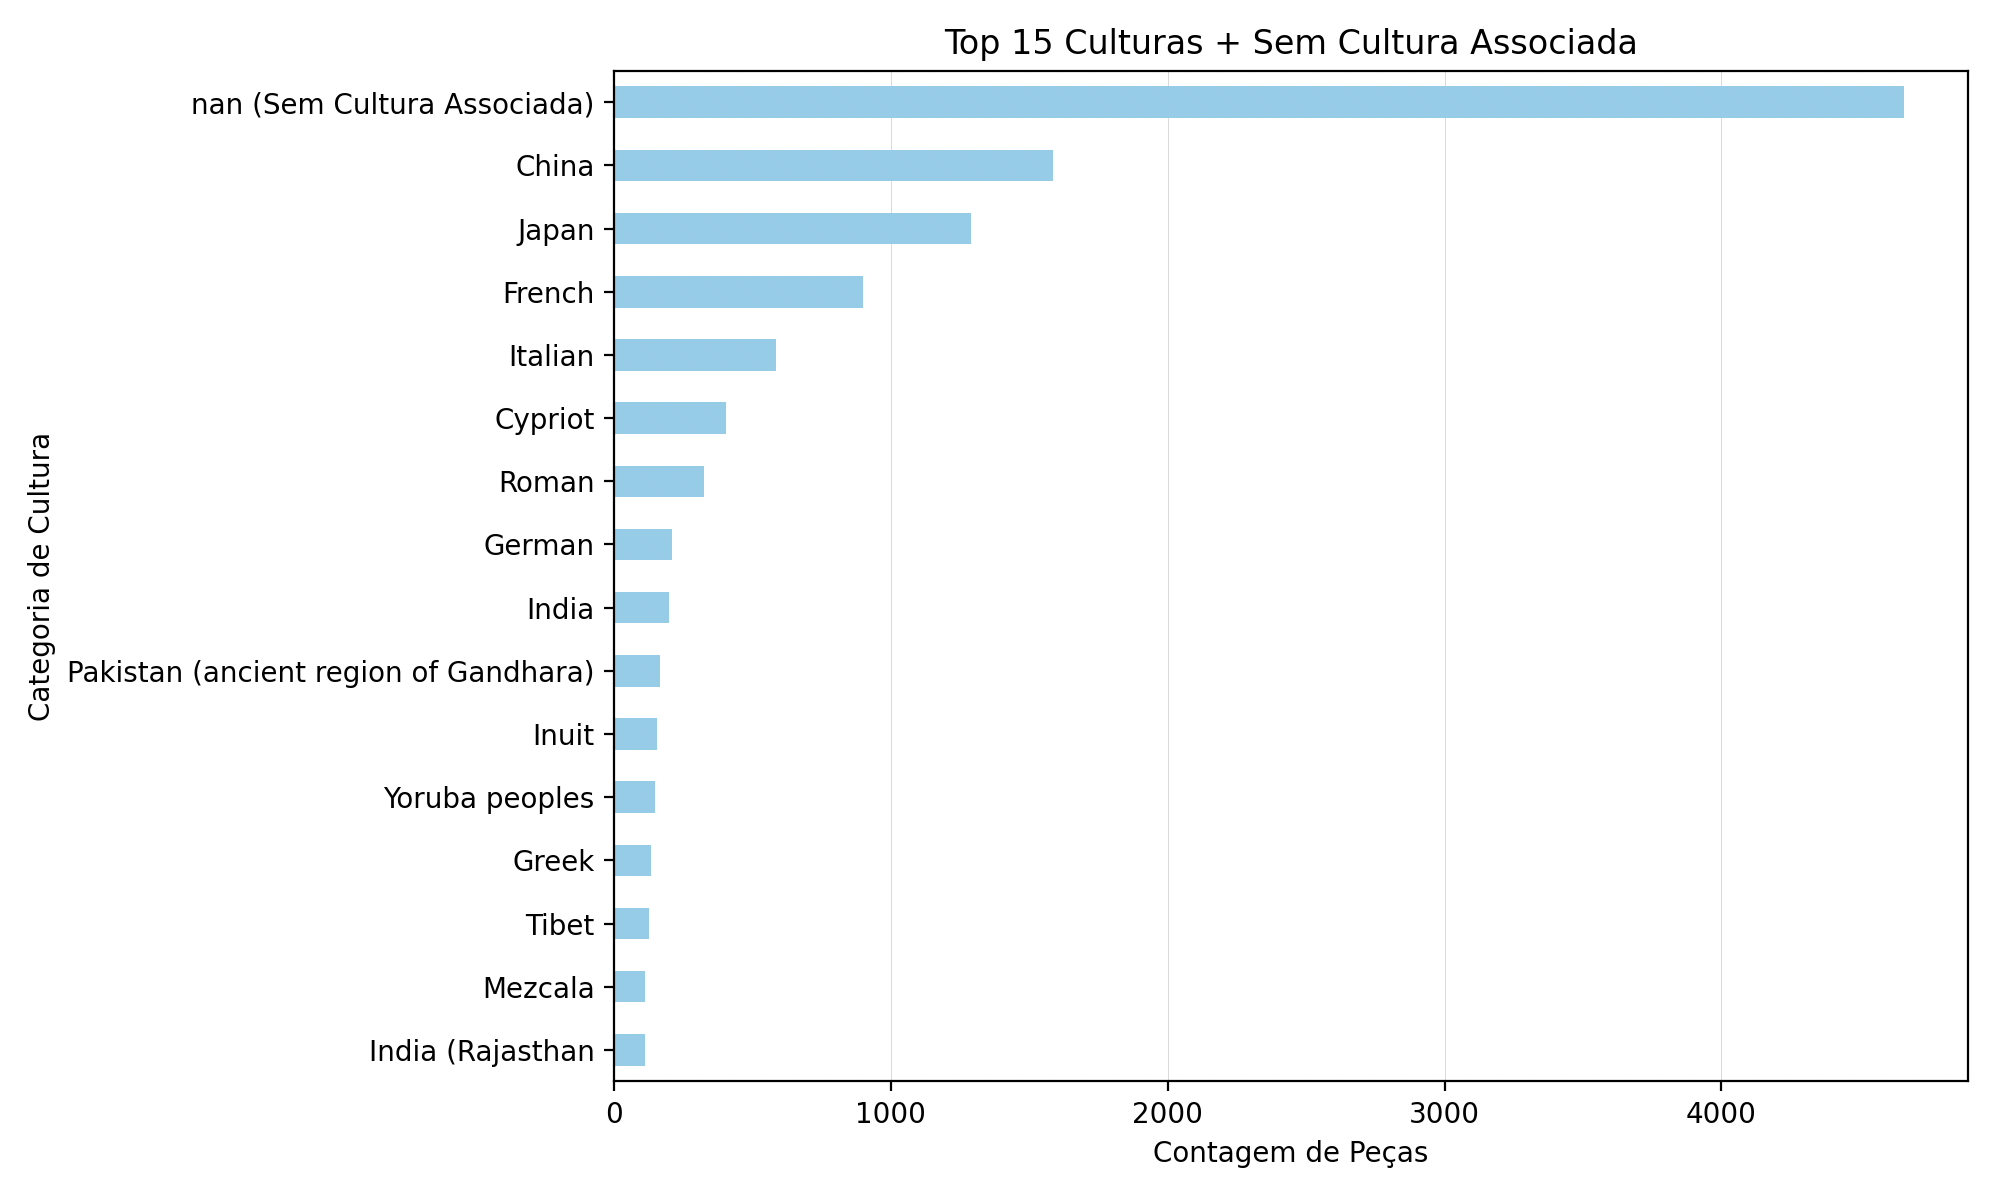
\includegraphics[width=0.8\textwidth]{../imagens/variaveis/Culture.png}
    \caption{Top 15 Culturas presentes no acervo e obras sem cultura associada.}
    \label{fig:cultura_panorama}
\end{figure}

O gráfico acima (Figura~\ref{fig:cultura_panorama}) apresenta a distribuição das principais culturas atribuídas pelo MET às obras de arte analisadas, considerando o recorte de esculturas e pinturas. Observa-se uma predominância de culturas europeias e asiáticas, com destaque para as categorias "China", "Japan", "French", "Italian" e "Cypriot". Essa concentração evidencia uma forte representação artística ligada a polos históricos de produção com tradição de preservação, isto é, culturas influentes na história mundial que demonstraram grande interesse e zelo pela arte. Além disso, esse gráfico também reflete o perfil de aquisição do Metropolitan Museum of Art, que tradicionalmente privilegiou obras oriundas de regiões valorizadas pelo colonialismo ocidental \cite{metMakingTheMet}.

Entretanto, é indispensável comentar o grande número de obras sem cultura associada, o que evidencia uma lacuna na base de dados disponibilizada pelo museu. Essa ausência pode ser decorrente da escassez de informações suficientes para uma identificação precisa, ou da priorização curatorial por outros critérios classificatórios. De qualquer forma, essa ausência limita parte da análise comparativa entre culturas e materiais. Ainda assim, a predominância de culturas com forte identidade material e técnica, como as mencionadas acima, fornece uma base consistente para as explorações da hipótese 1, que serão desenvolvidas a seguir.

\subsubsection{Os Materiais em Cada Cultura}

\begin{figure}[H]
    \centering
    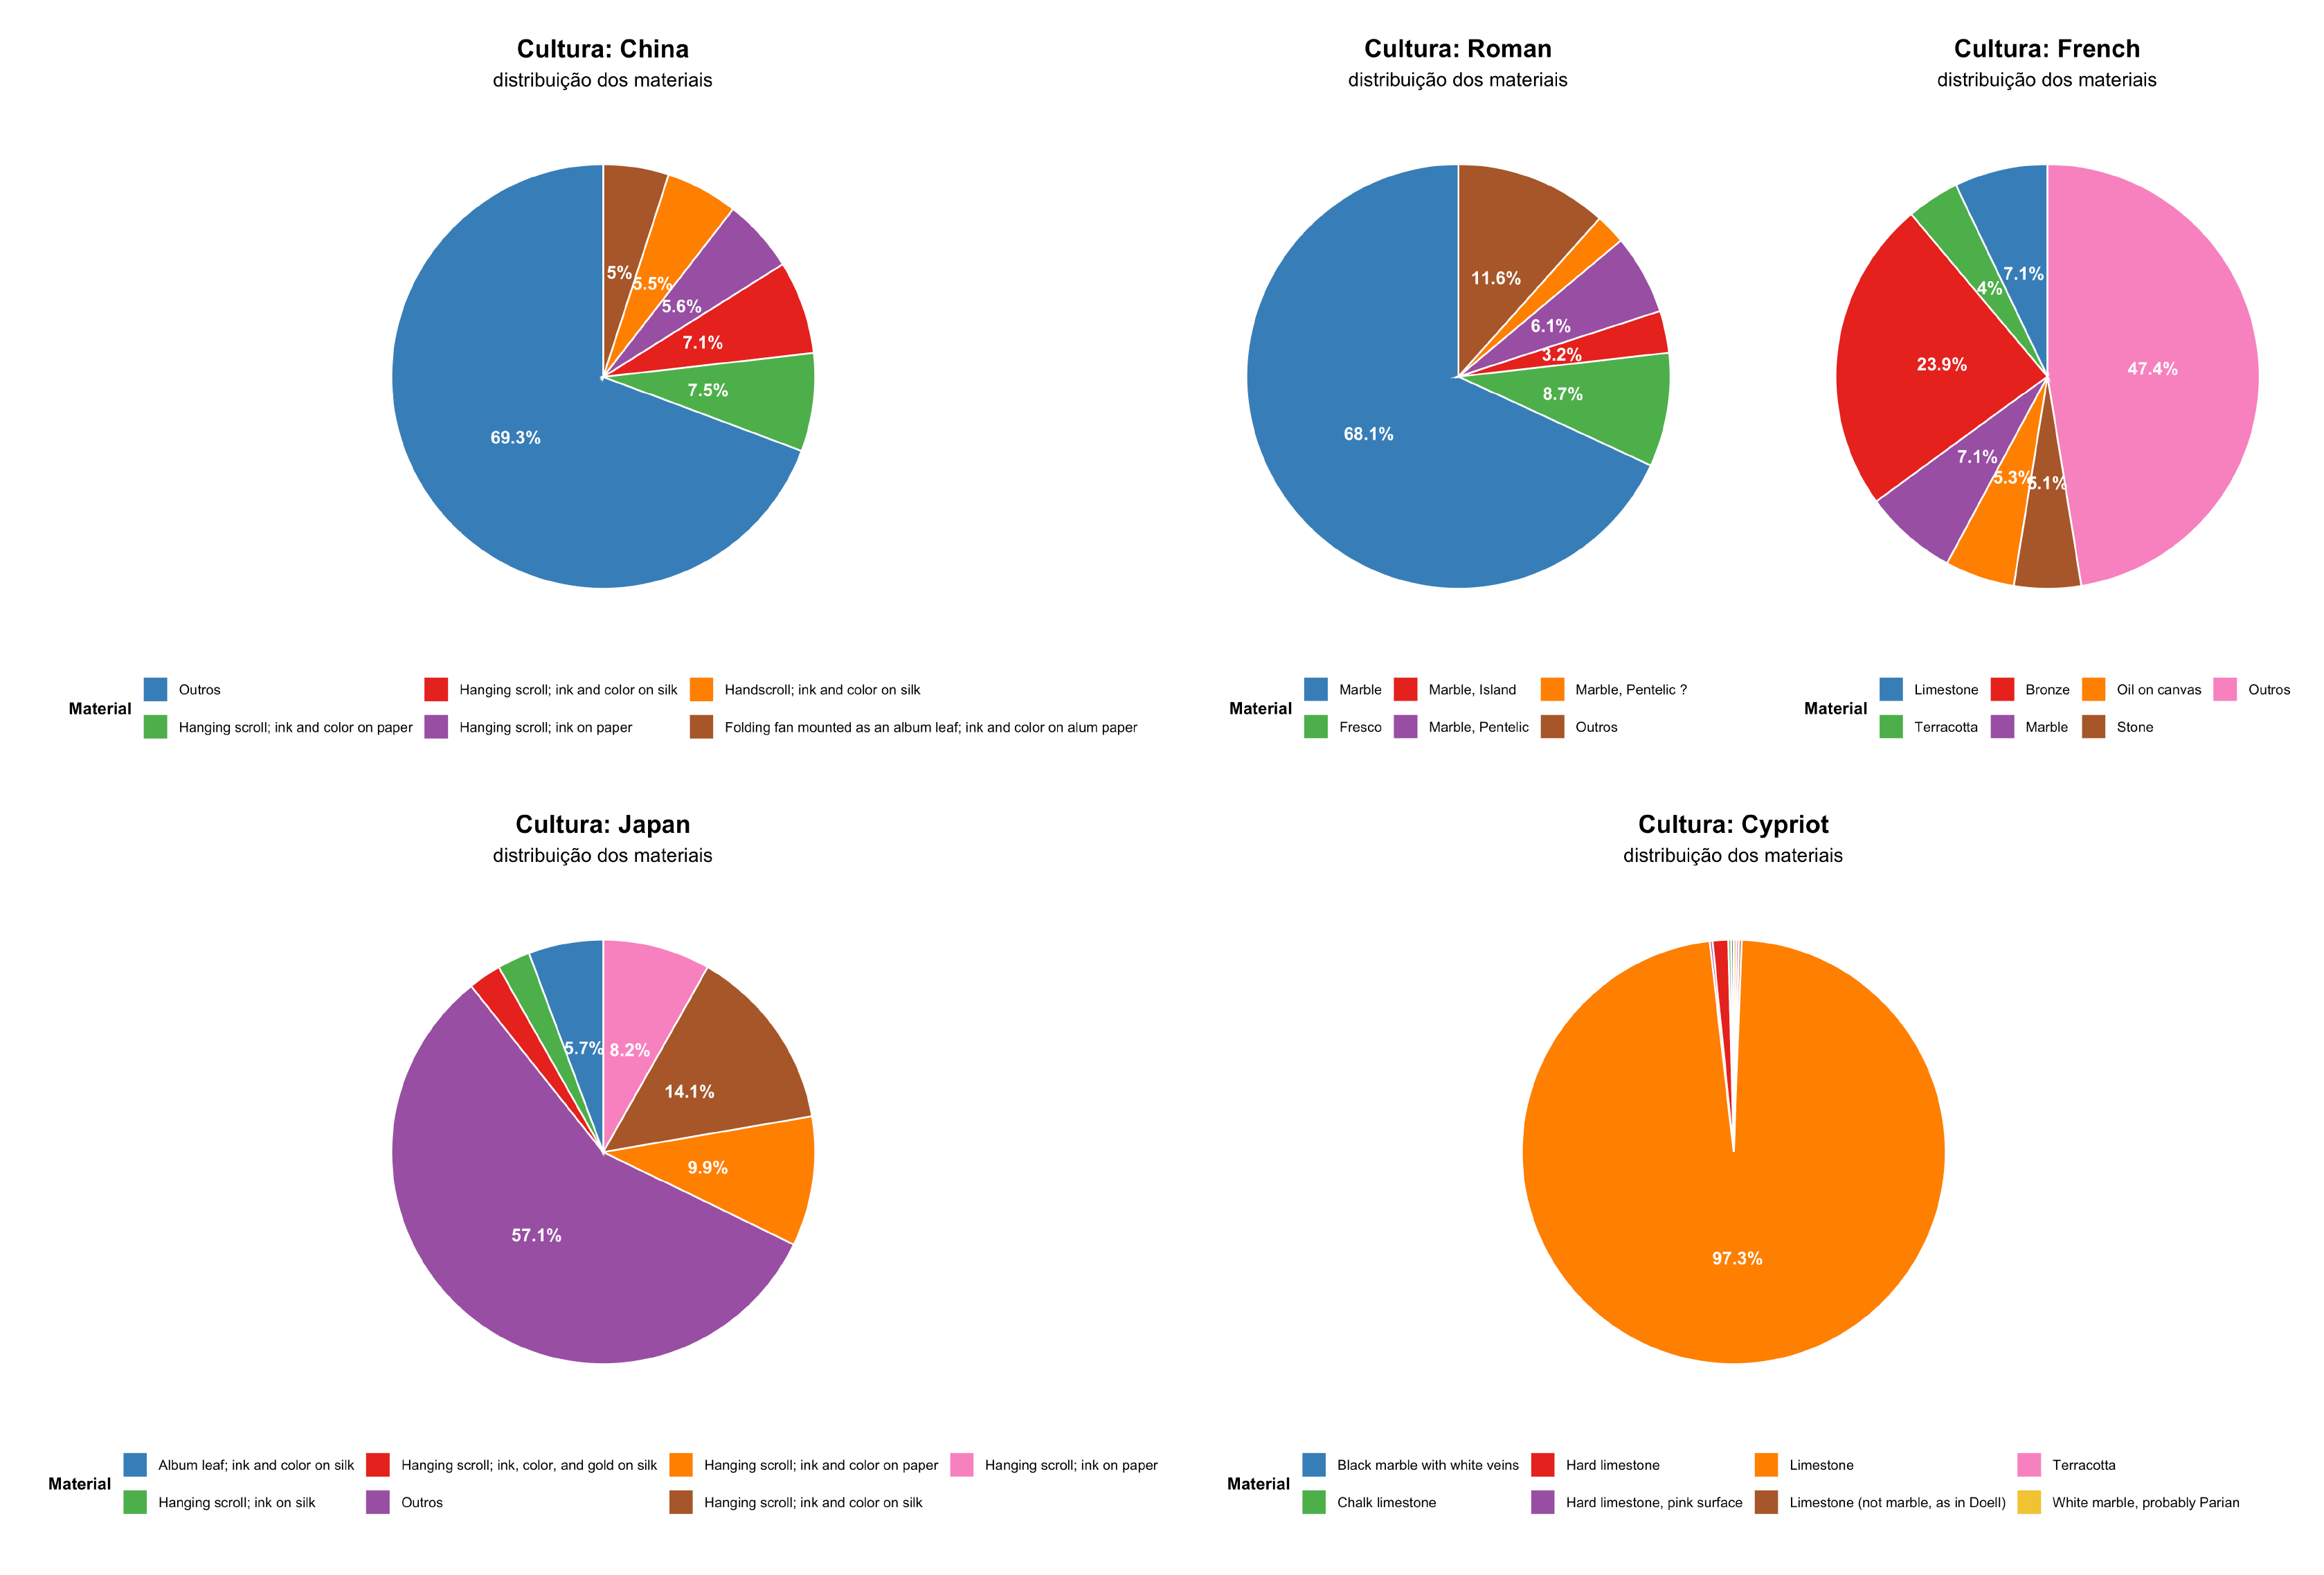
\includegraphics[width=1\textwidth]{../imagens/variaveis/resumo_culturas.png}
    \caption{Distribuição de materiais nas principais culturas analisadas.}
    \label{fig:materiais_culturas}
\end{figure}

Os gráficos (Figura~\ref{fig:materiais_culturas}) acima ilustram os materiais predominantes utilizados nas obras das culturas "China", "Japan", "Roman", "French" e "Cypriot". Analisando-os, observam-se padrões coerentes com os contextos geográficos e tecnológicos de cada civilização. Nas culturas chinesa e japonesa, por exemplo, nota-se o uso frequente de seda, papel e tinta --- materiais ligados à tradição artística asiática e à disponibilidade de recursos naturais locais. Já nas obras romanas e cipriotas, predominam materiais como mármore, calcário e cerâmica, compatíveis com a extração mineral abundante no Mediterrâneo e com as técnicas escultóricas clássicas. A cultura francesa, por sua vez, se destaca pelo uso de óleo sobre tela, consolidado como o meio artístico (do inglês \textit{medium}) dominante da pintura europeia desde o Renascimento.
Esses dados fortalecem a hipótese de que as tendências materiais em obras artísticas estão relacionadas às possibilidades físicas e técnicas disponíveis em cada território e época, moldando a identidade visual de cada cultura representada no acervo.

\subsubsection{Visão geral dos materiais no acervo}

\begin{figure}[H]
    \centering
    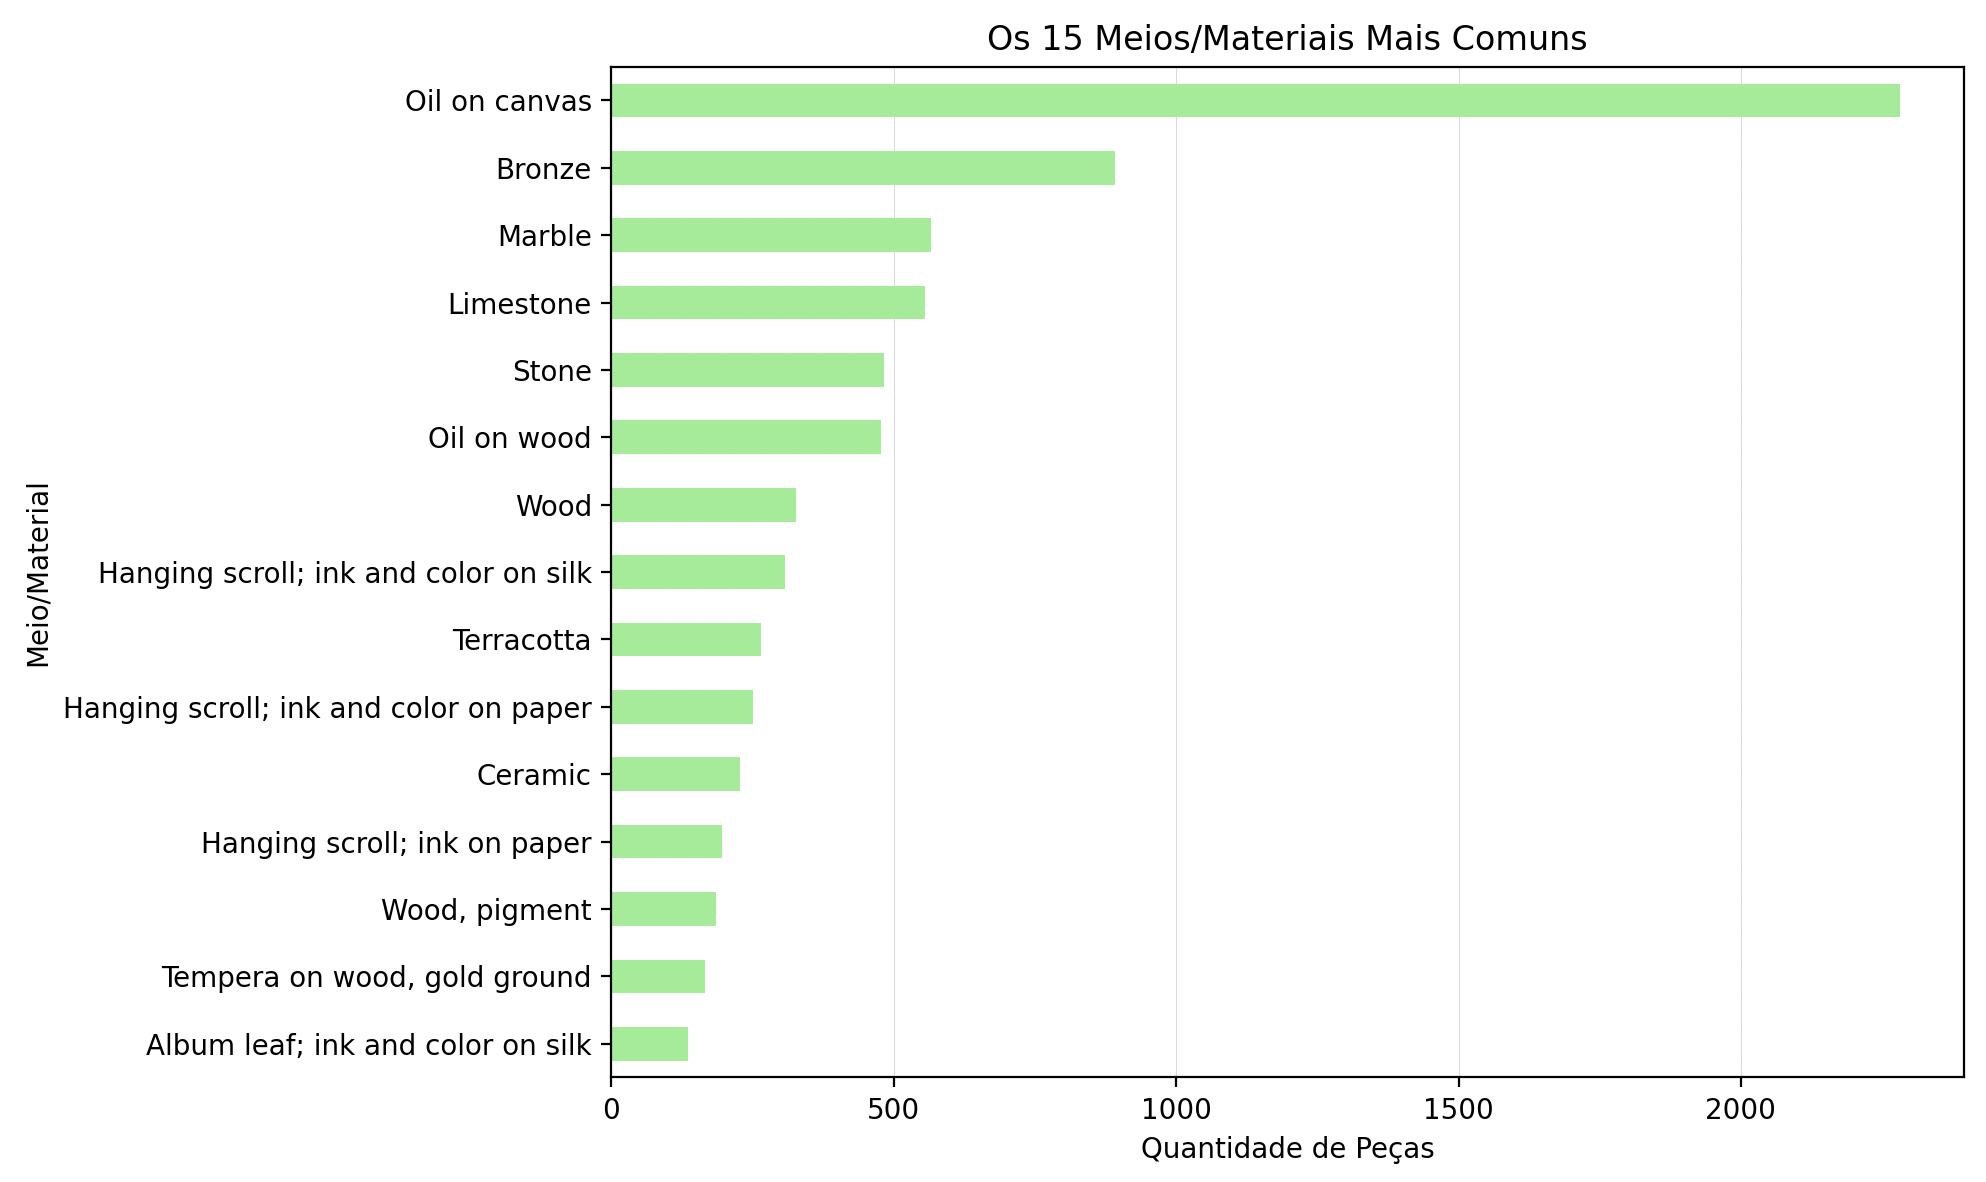
\includegraphics[width=0.9\textwidth]{../imagens/variaveis/Medium.png} % Presumindo que Medium.png está em ../imagens/variaveis/
    \caption{Os 15 Meios/Materiais Mais Comuns no acervo analisado.}
    \label{fig:materiais_geral}
\end{figure}

	A figura acima (Figura~\ref{fig:materiais_geral}) oferece uma visão abrangente dos materiais empregados nas pinturas e esculturas do acervo do museu. Nela, observa-se tanto o predomínio de tradições culturais ocidentais centrais – europeias e norte-americanas – quanto o efeito de seus ambientes físicos e geográficos, que favoreceram a coleta e a circulação desses cânones artísticos.
	Sobressai-se, em particular, a magnitude do óleo sobre tela. Esse meio não apenas supera todas as demais técnicas de pintura, mas também ultrapassa, em número de obras, a soma de diversos materiais usados em esculturas. A distância que o separa de outras formas de pintura, aparecendo somente na sexta posição no ranking, reforça esse contraste.
	Esse domínio remonta às condições materiais e urbanas da Europa: a disponibilidade de linho, as oficinas concentradas em grandes centros e o comércio marítimo permitiram que a tela se firmasse como suporte preferencial desde o Renascimento. A forte demanda por obras renascentistas, barrocas e românticas, circuladas por colecionadores, consolidou esse viés.
	Finalmente, aspectos técnicos e ambientais também exerceram papel decisivo. Em climas variados, o óleo sobre tela provou-se durável; sua maleabilidade permite alto grau de detalhamento e transições cromáticas sutis; e, por ser mais leve que painéis de madeira, facilitou o transporte e a difusão em larga escala.

\subsection{A Popularidade e o Tempo: Investigando a Hipótese 2}
\subsubsection{Obras Em Destaque, o Que São?}

\begin{figure}[H]
    \centering
    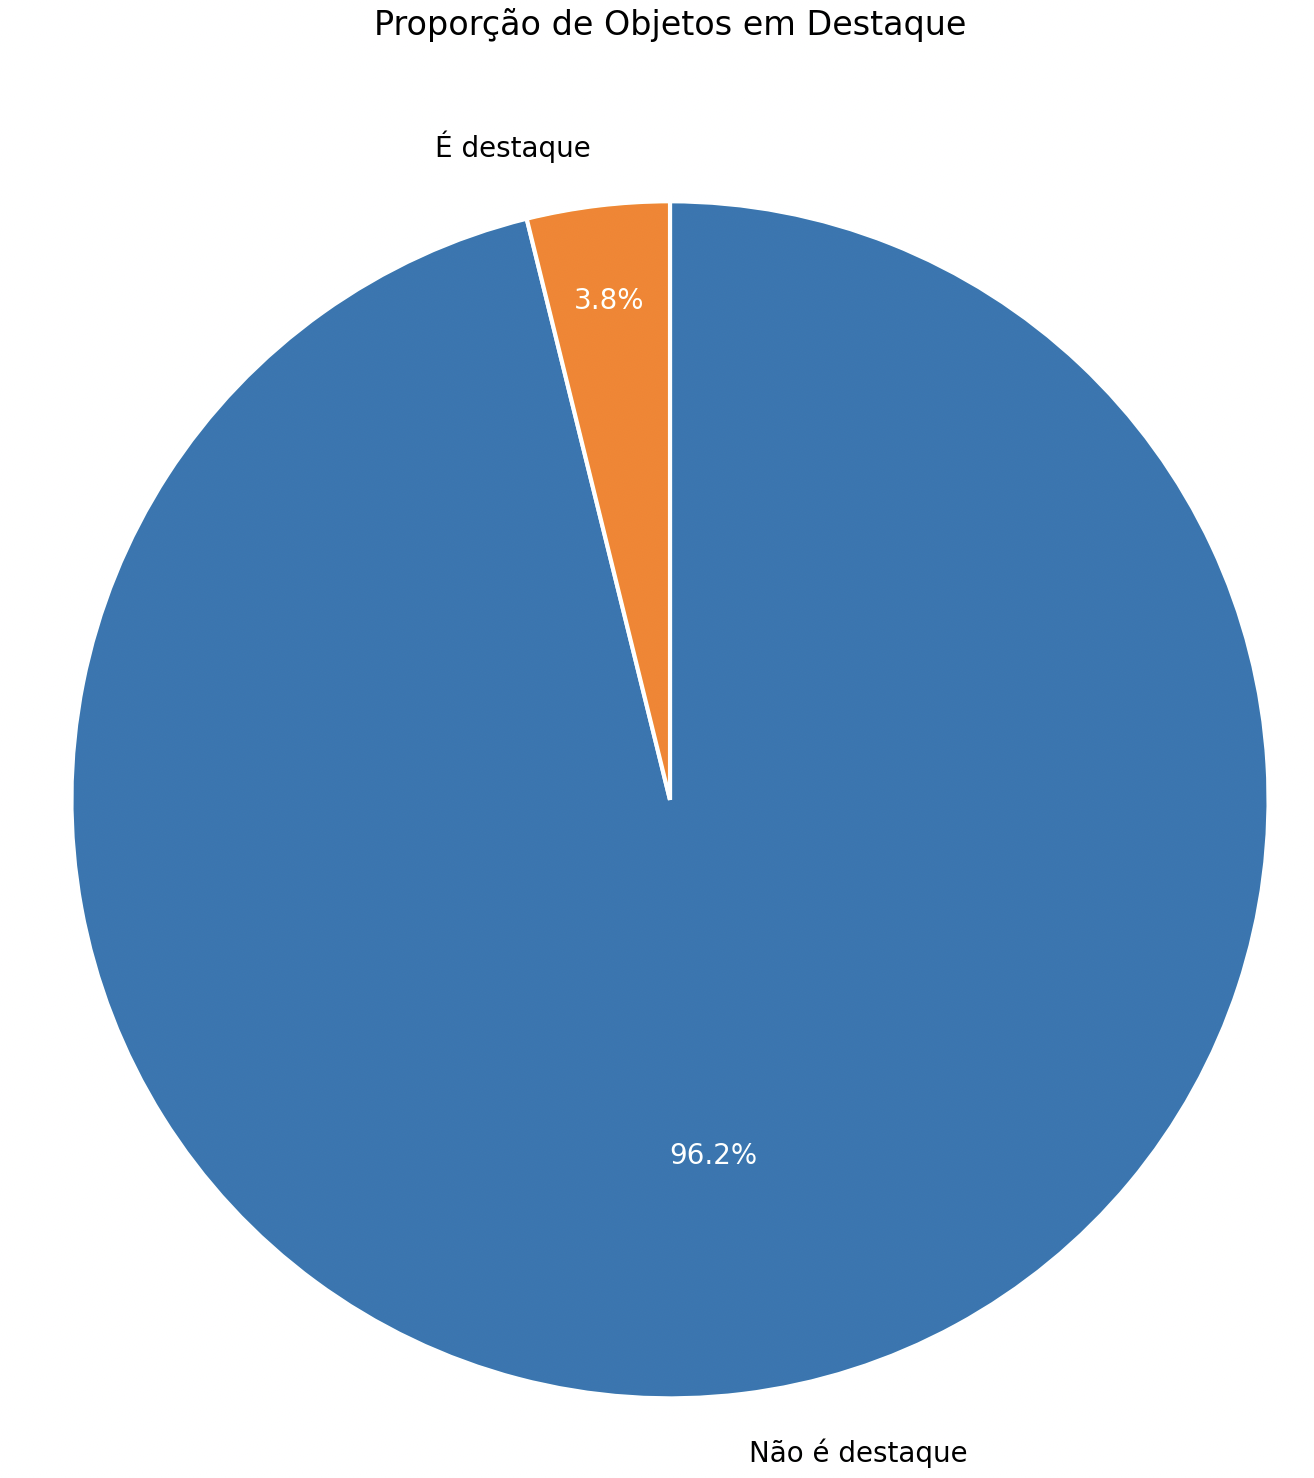
\includegraphics[width=0.4\textwidth]{../imagens/variaveis/IsHighlight.png}
    \caption{Proporção de obras em destaque no acervo de pinturas e esculturas.}
    \label{fig:ishighlight_prop}
\end{figure}

O gráfico acima (Figura~\ref{fig:ishighlight_prop}) apresenta a proporção de obras classificadas como "em destaque" no acervo analisado. Observa-se que apenas 3,8\% das esculturas e pinturas selecionadas recebem essa classificação, o que evidencia um critério curatorial restrito. O status de destaque, atribuído pelo próprio Metropolitan Museum of Art, indica obras consideradas especialmente relevantes, seja por seu valor histórico, estético, técnico ou por sua visibilidade em exposições. Neste trabalho, tal classification será utilizada como um indicador de popularidade, permitindo investigar quais características tendem a estar mais presentes nas obras destacadas, conforme propõe a hipótese 2.

\subsubsection{Análise do Tema de Obras em Destaque}

\begin{figure}[H]
    \centering
    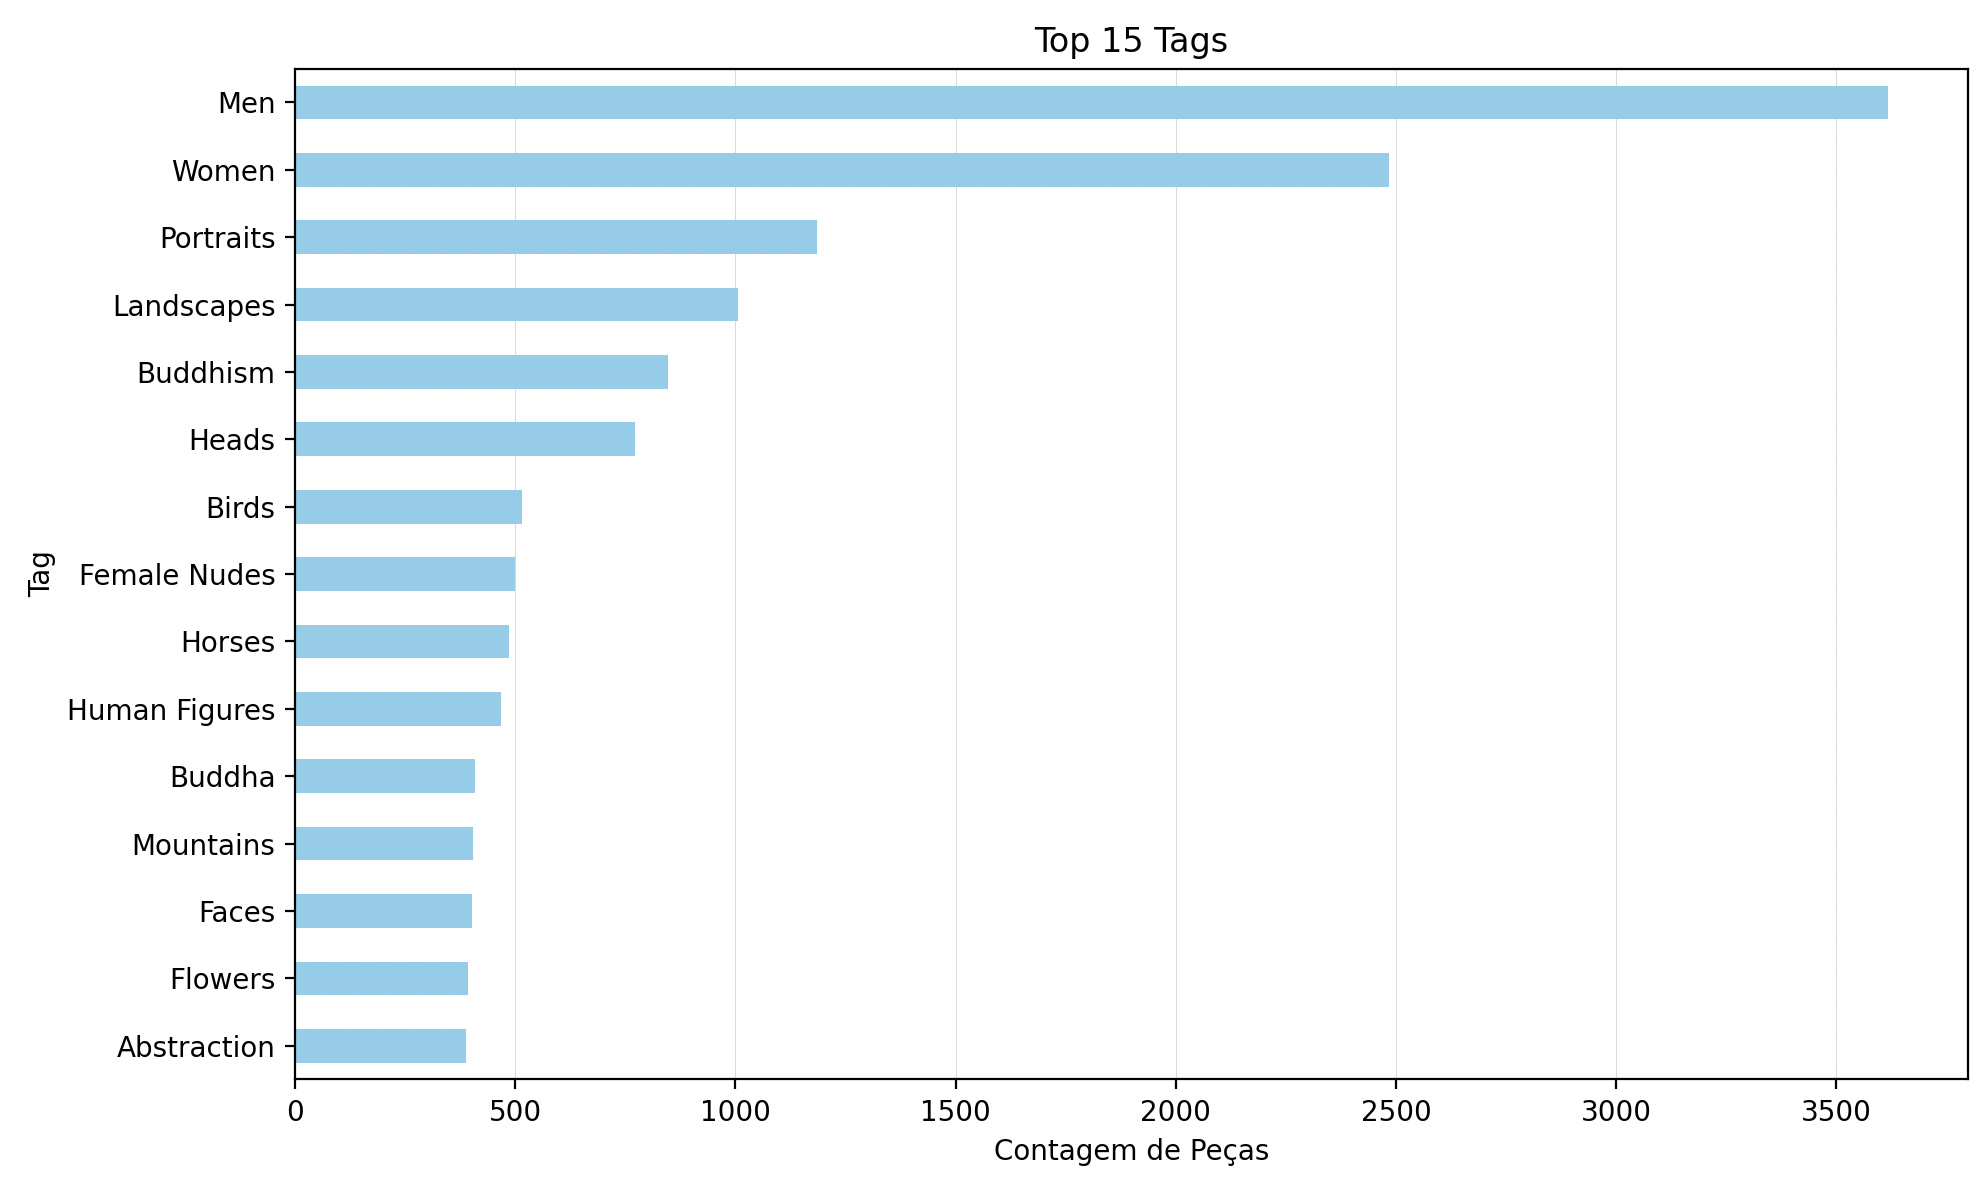
\includegraphics[width=0.7\textwidth]{../imagens/variaveis/Tags.png}
    \caption{Top 15 temas (tags) mais frequentes no acervo de pinturas e esculturas.}
    \label{fig:tags_geral}
\end{figure}

\begin{figure}[H]
    \centering
    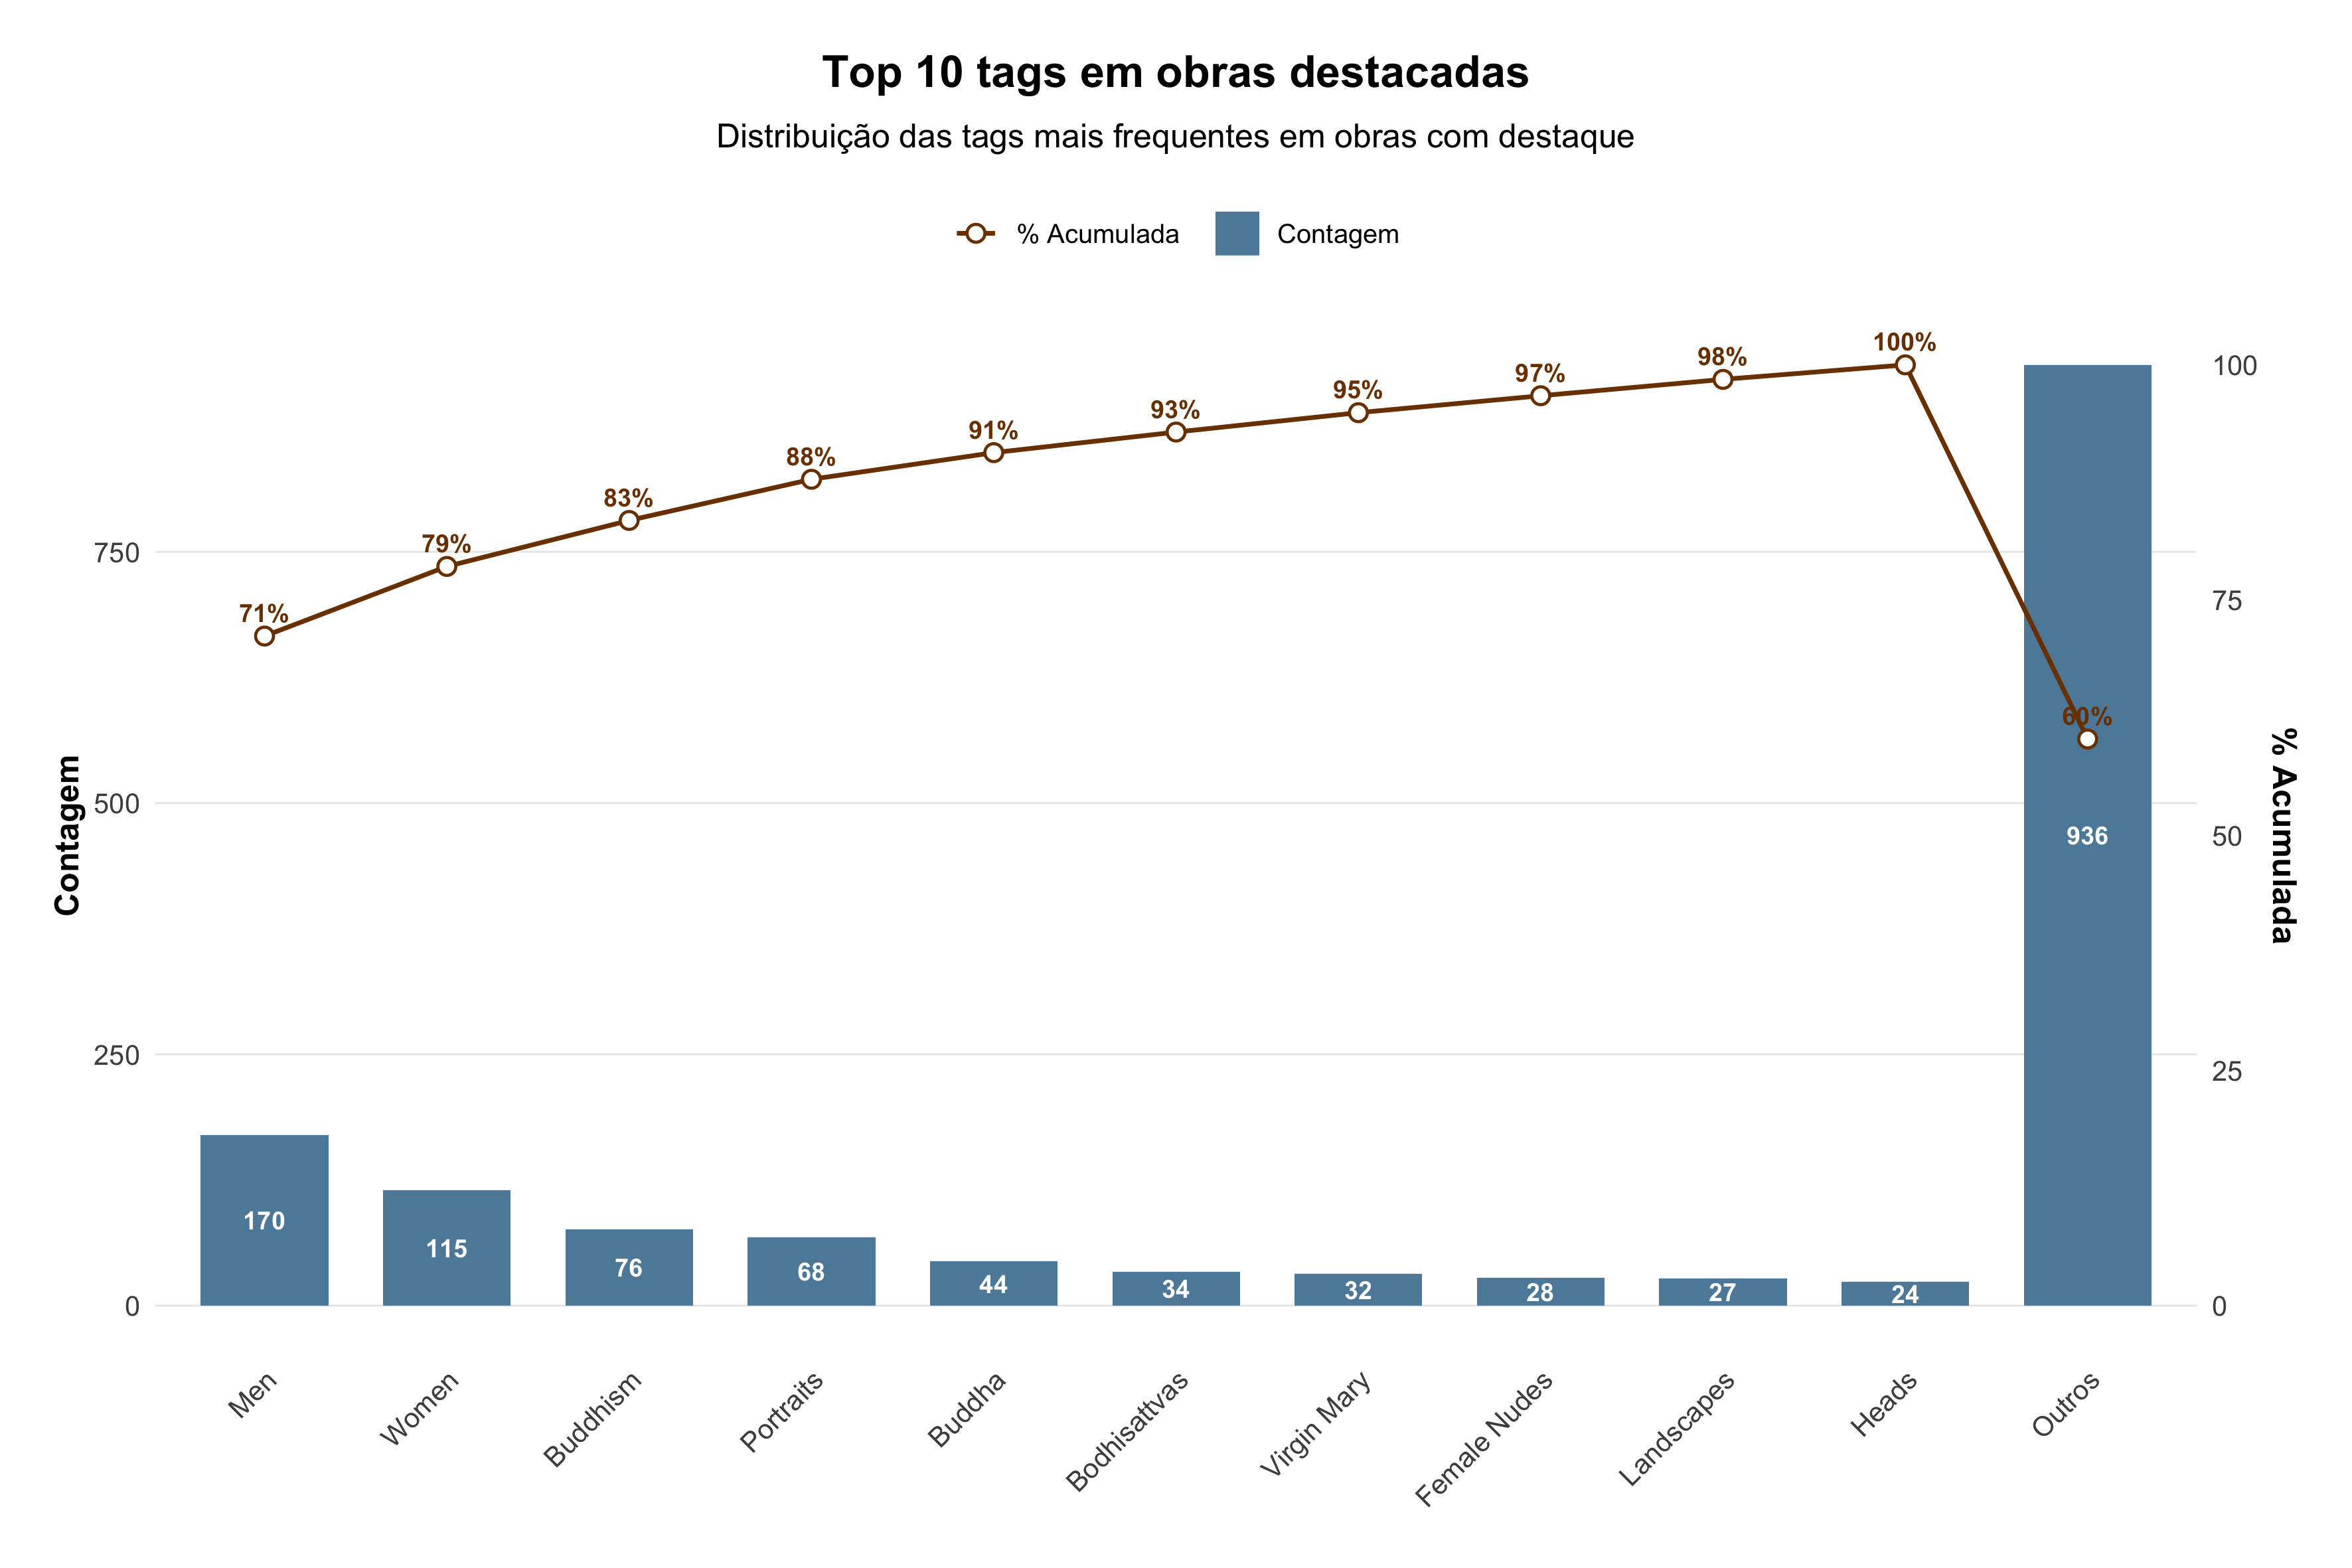
\includegraphics[width=0.7\textwidth]{../imagens/pareto_tags_highlight.png}
    \caption{Distribuição de Pareto dos temas (tags) mais frequentes em obras destacadas.}
    \label{fig:pareto_tags_highlight}
\end{figure}

Nesses gráficos (Figura~\ref{fig:tags_geral} e Figura~\ref{fig:pareto_tags_highlight}), observam-se os temas que aparecem com mais frequência nas obras analisadas, assim como aqueles que predominam entre as obras classificadas como "em destaque". No conjunto geral do acervo, destacam-se temas relacionados a gênero e retratos (como "Men", "Women" e "Portraits"), seguidos por temáticas religiosas. Isso evidencia uma ampla representação de elementos humanos e espirituais, populares na produção artística ao longo da história.
Quando se observa apenas o recorte das obras em destaque, percebe-se uma mudança sutil no padrão de recorrência. A curva de Pareto mostra que os temas mais frequentes entre essas obras possuem forte conteúdo religioso, histórico e humano, ao contrário de representações como flores, montanhas e abstrações, que aparecem com maior frequência entre as 15 \textit{tags} mais comuns no geral. Isso sugere uma preferência curatorial por obras que, além de seu valor estético, carregam narrativas culturalmente densas. Esses dados reforçam a noção de que, para uma obra ser considerada "em destaque", não basta estar relacionada a temáticas recorrentes --- é preciso também que apresente uma força simbólica e histórica atribuída a determinados conteúdos.

\subsubsection{Dimensões Físicas}

\begin{figure}[H]
    \centering
    \begin{subfigure}[b]{0.48\textwidth}
        \centering
        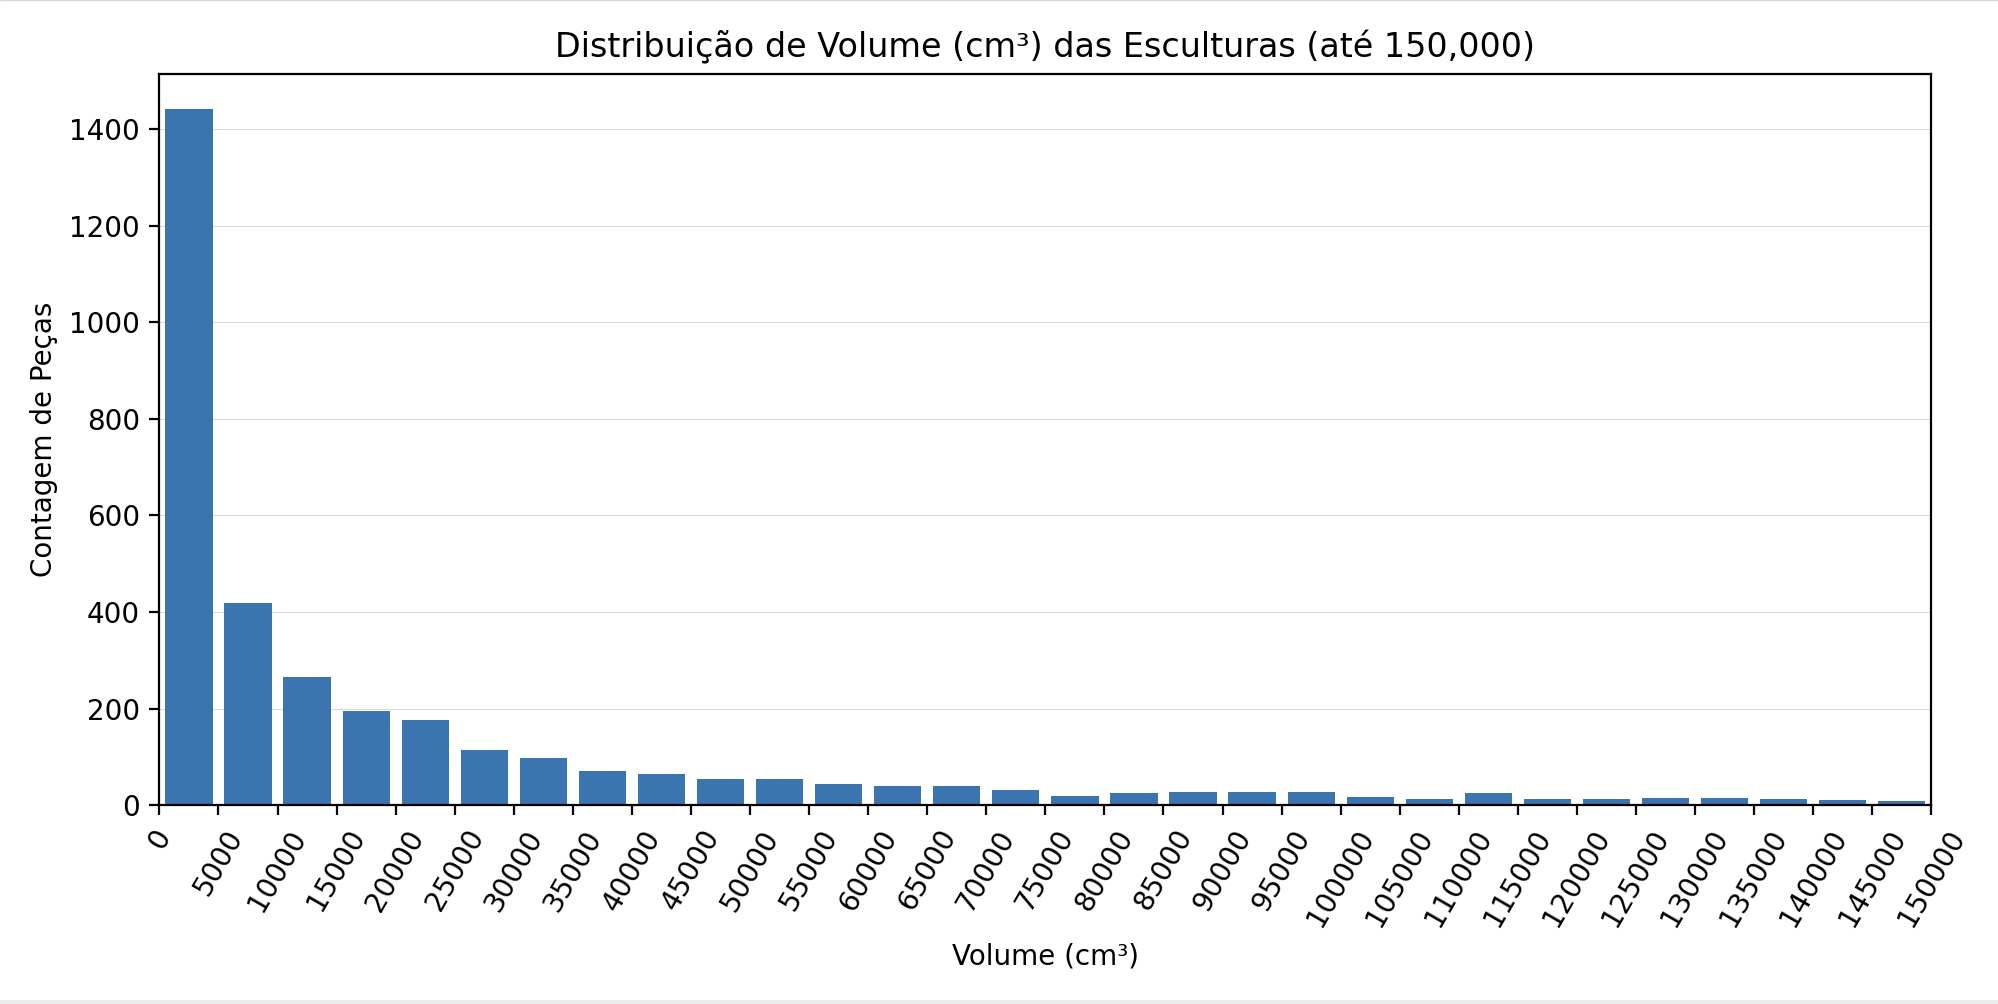
\includegraphics[width=\textwidth]{../imagens/variaveis/DimensoesEsculturasVolume.png}
        \caption{Distribuição de Volume das Esculturas (até 150,000 cm³).}
        \label{fig:dim_esculturas}
    \end{subfigure}
    \hfill % Espaçamento horizontal
    \begin{subfigure}[b]{0.48\textwidth}
        \centering
        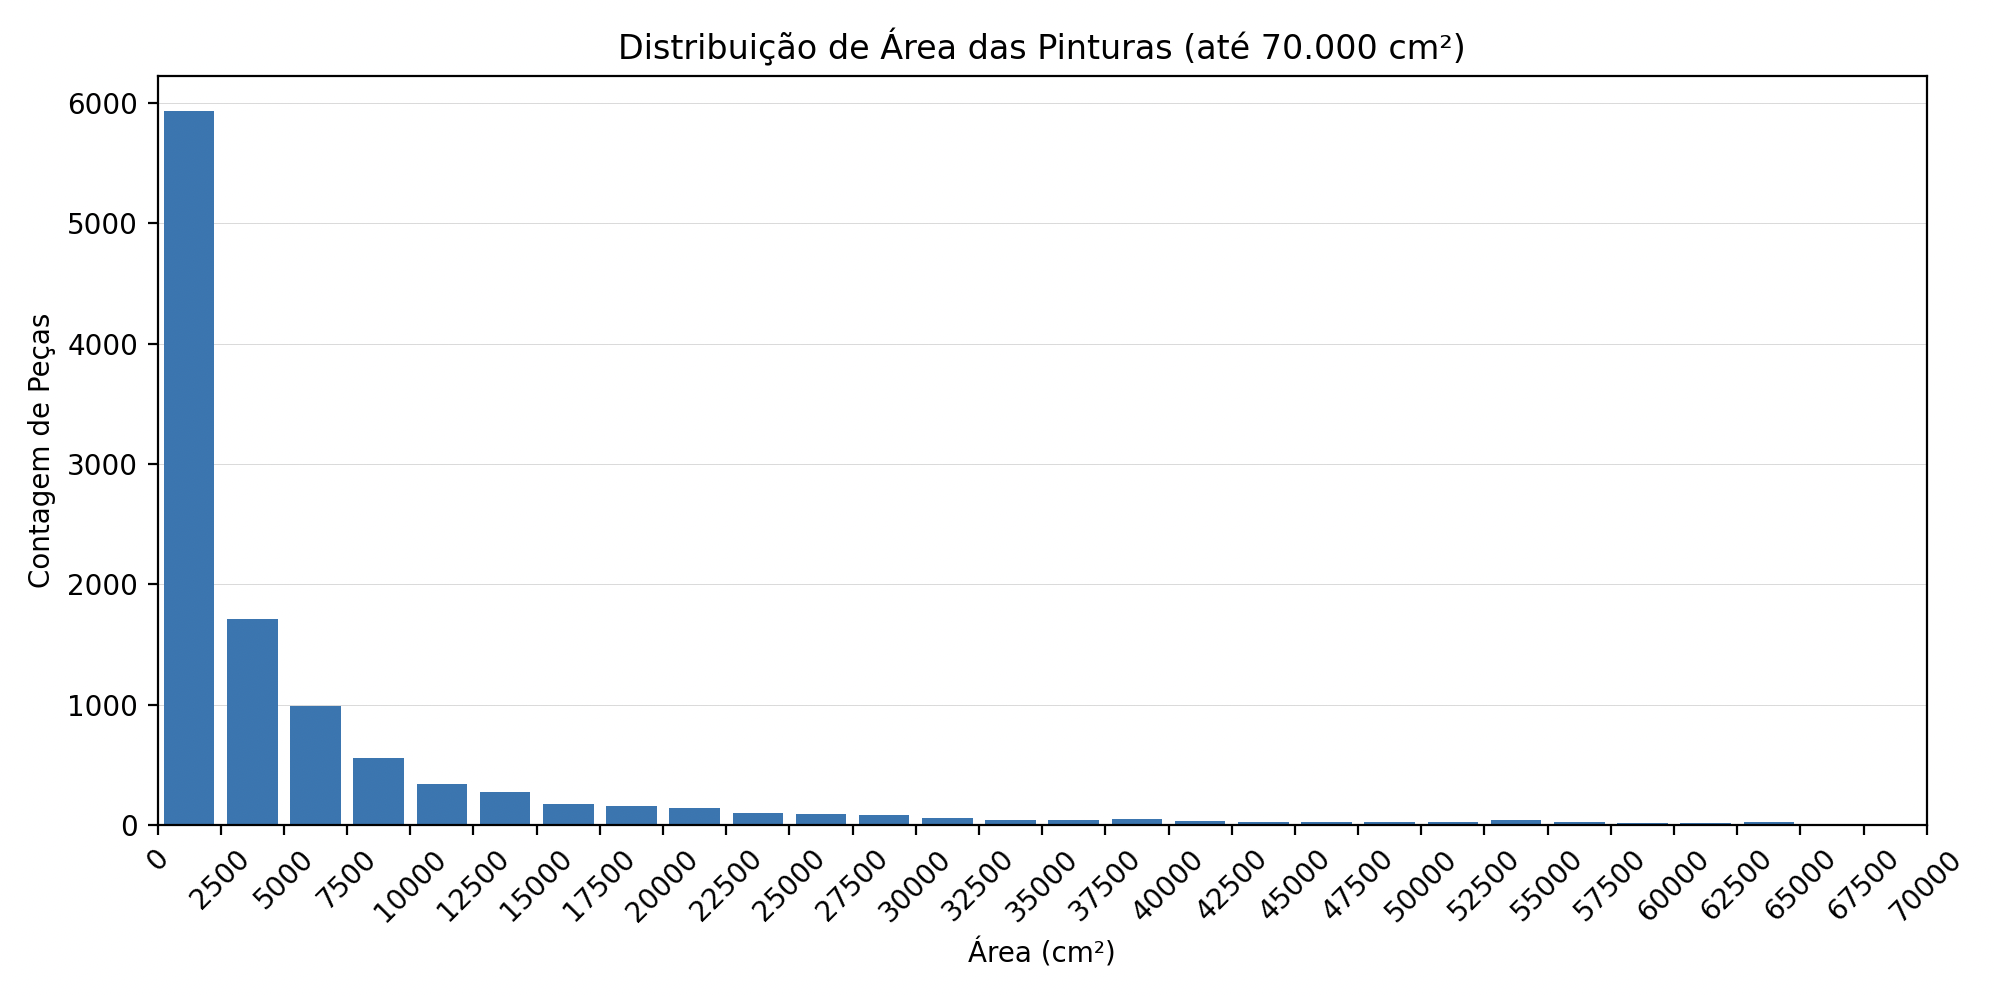
\includegraphics[width=\textwidth]{../imagens/variaveis/DimensoesPinturasArea.png} 
        \caption{Distribuição de Área das Pinturas (até 70,000 cm²).}
        \label{fig:dim_pinturas}
    \end{subfigure}
    \caption{Distribuição das dimensões físicas de esculturas e pinturas no acervo.}
    \label{fig:dimensoes_fisicas}
\end{figure}

Observa-se, ao analisar os gráficos "Distribuição de Área das Pinturas" (Figura~\ref{fig:dim_pinturas}) e "Distribuição de Volume das Esculturas" (Figura~\ref{fig:dim_esculturas}), que a distribuição das respectivas medidas é bastante assimétrica, concentrando-se, principalmente, nos valores mais baixos. Na prática, isso indica que a maioria das pinturas e esculturas do museu é de pequeno porte, com poucas exceções de peças muito grandes.

\begin{figure}[H]
    \centering
    \begin{subfigure}[b]{0.48\textwidth}
        \centering
        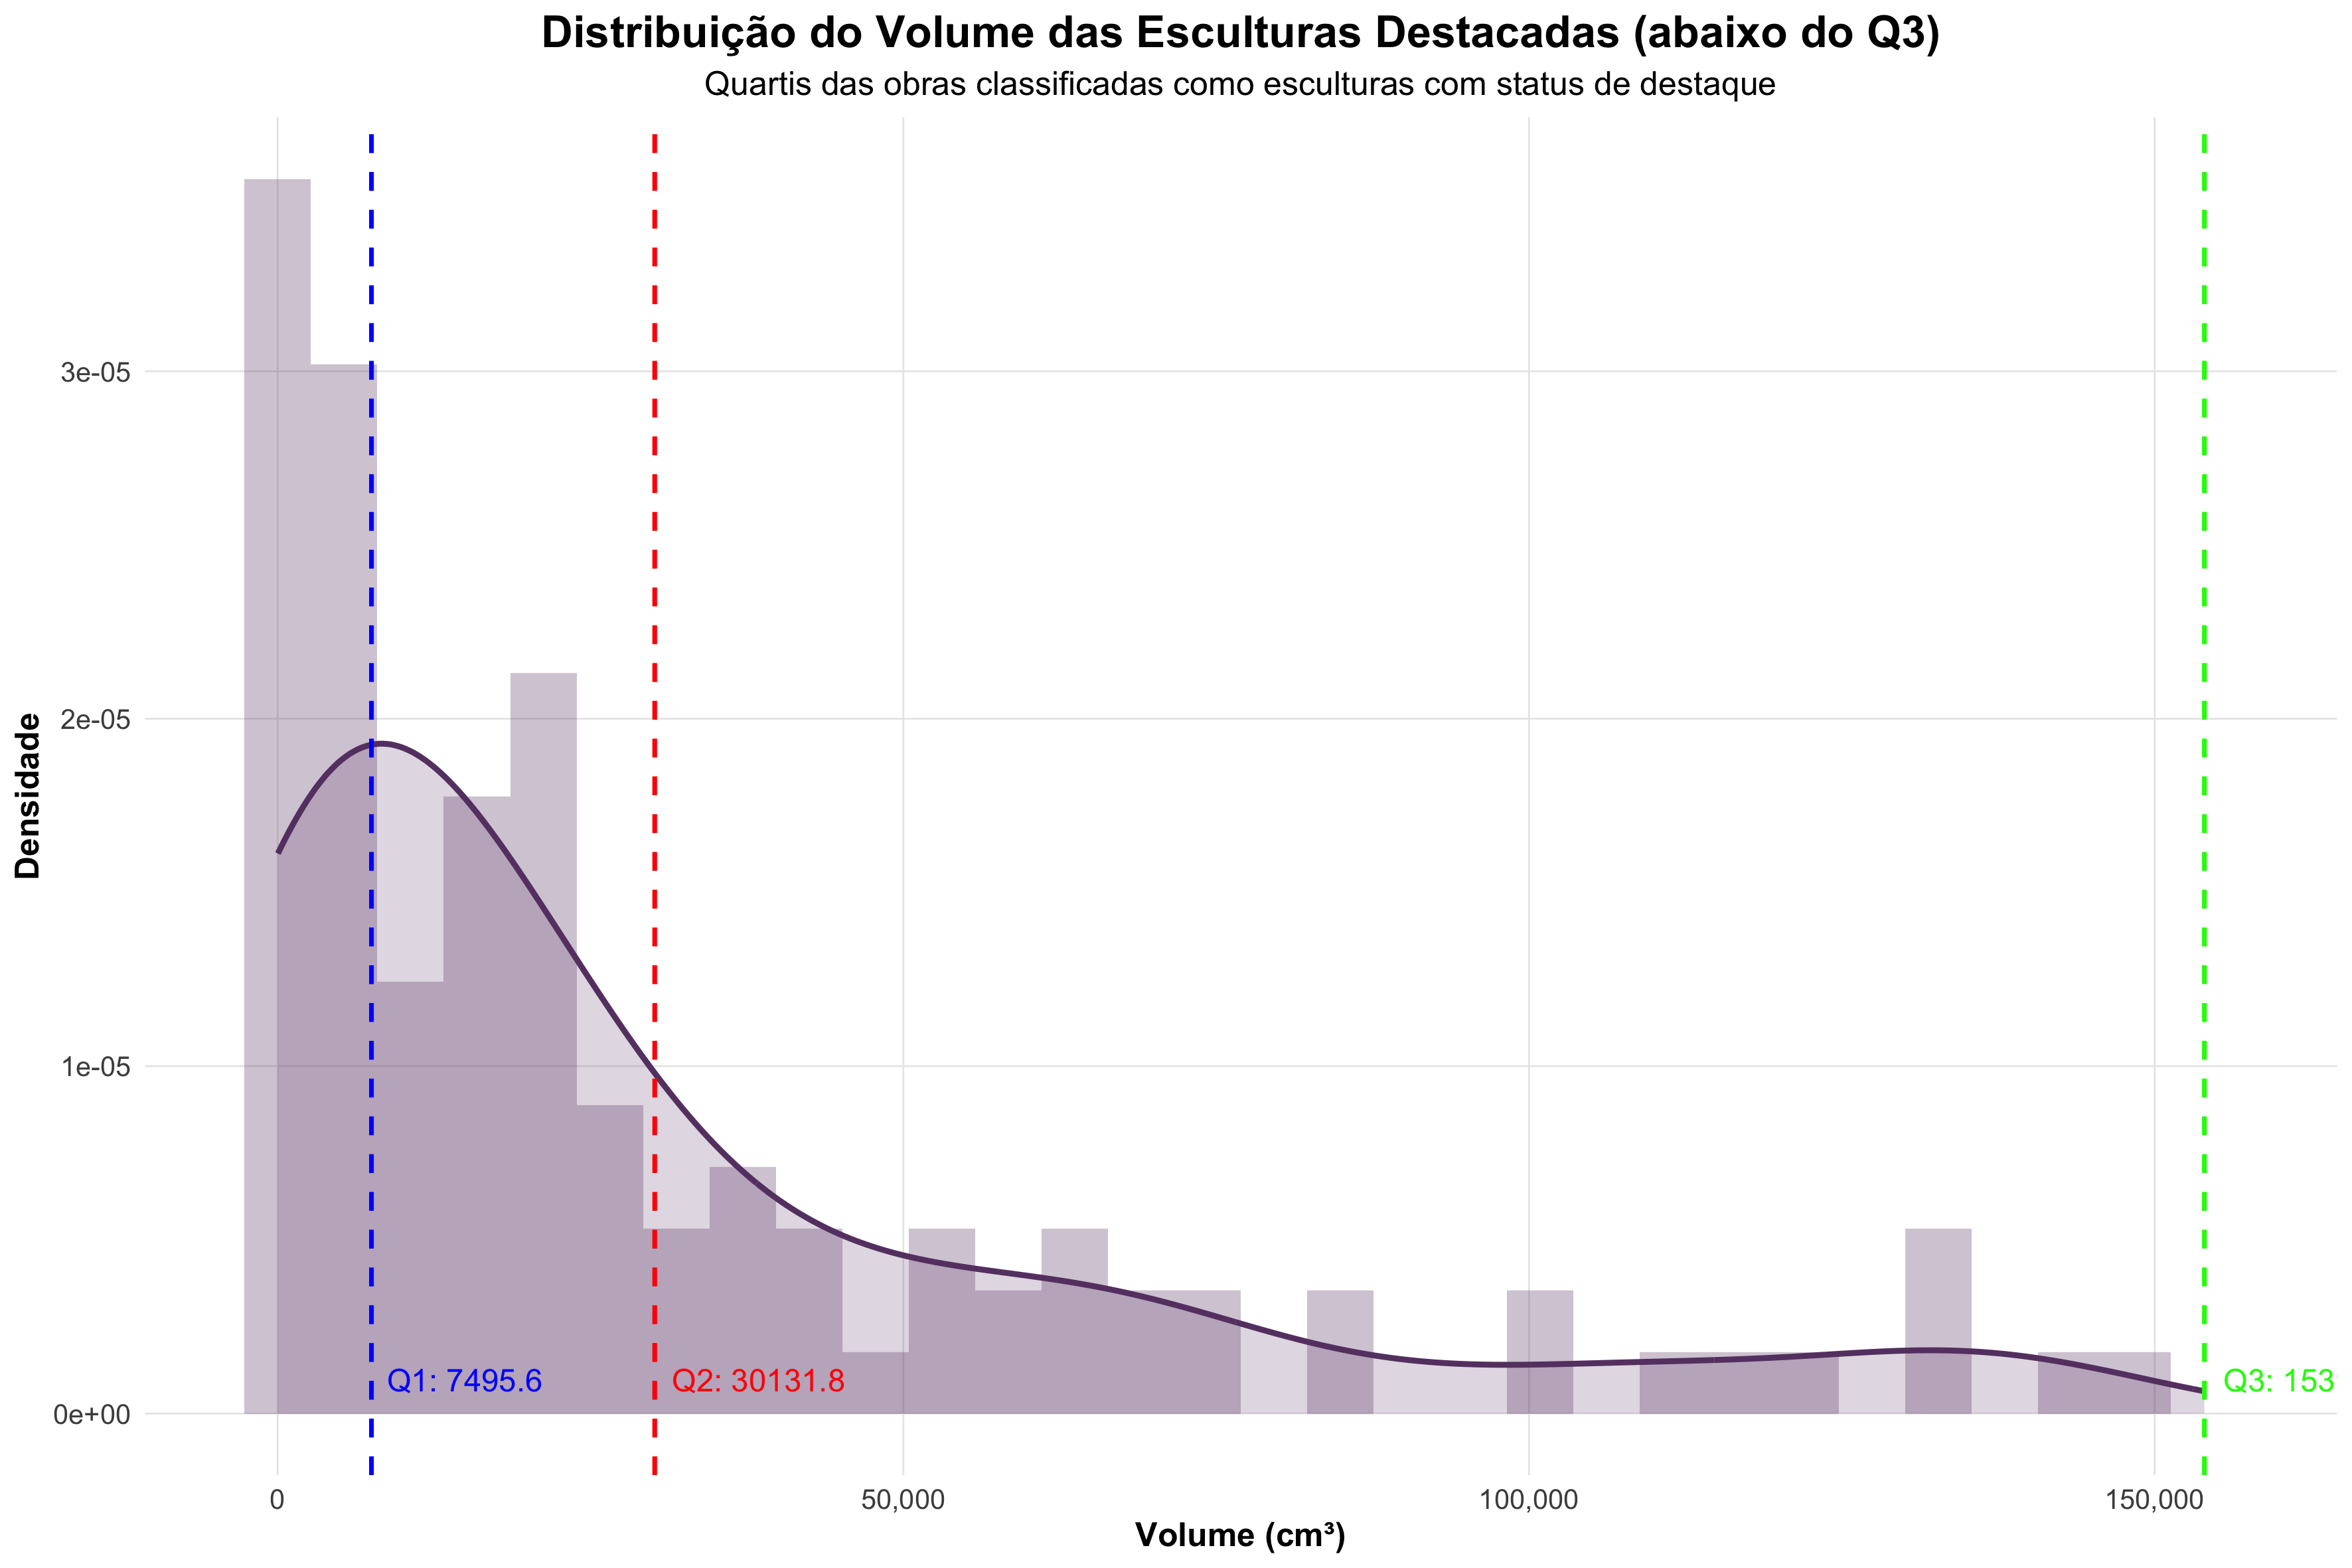
\includegraphics[width=\textwidth]{../imagens/densidade_esculturas_highlight_q3.png} 
        \caption{Densidade do Volume das Esculturas em Destaque (abaixo do Q3).}
        \label{fig:densidade_esculturas_highlight}
    \end{subfigure}
    \hfill % Espaçamento horizontal
    \begin{subfigure}[b]{0.48\textwidth}
        \centering
        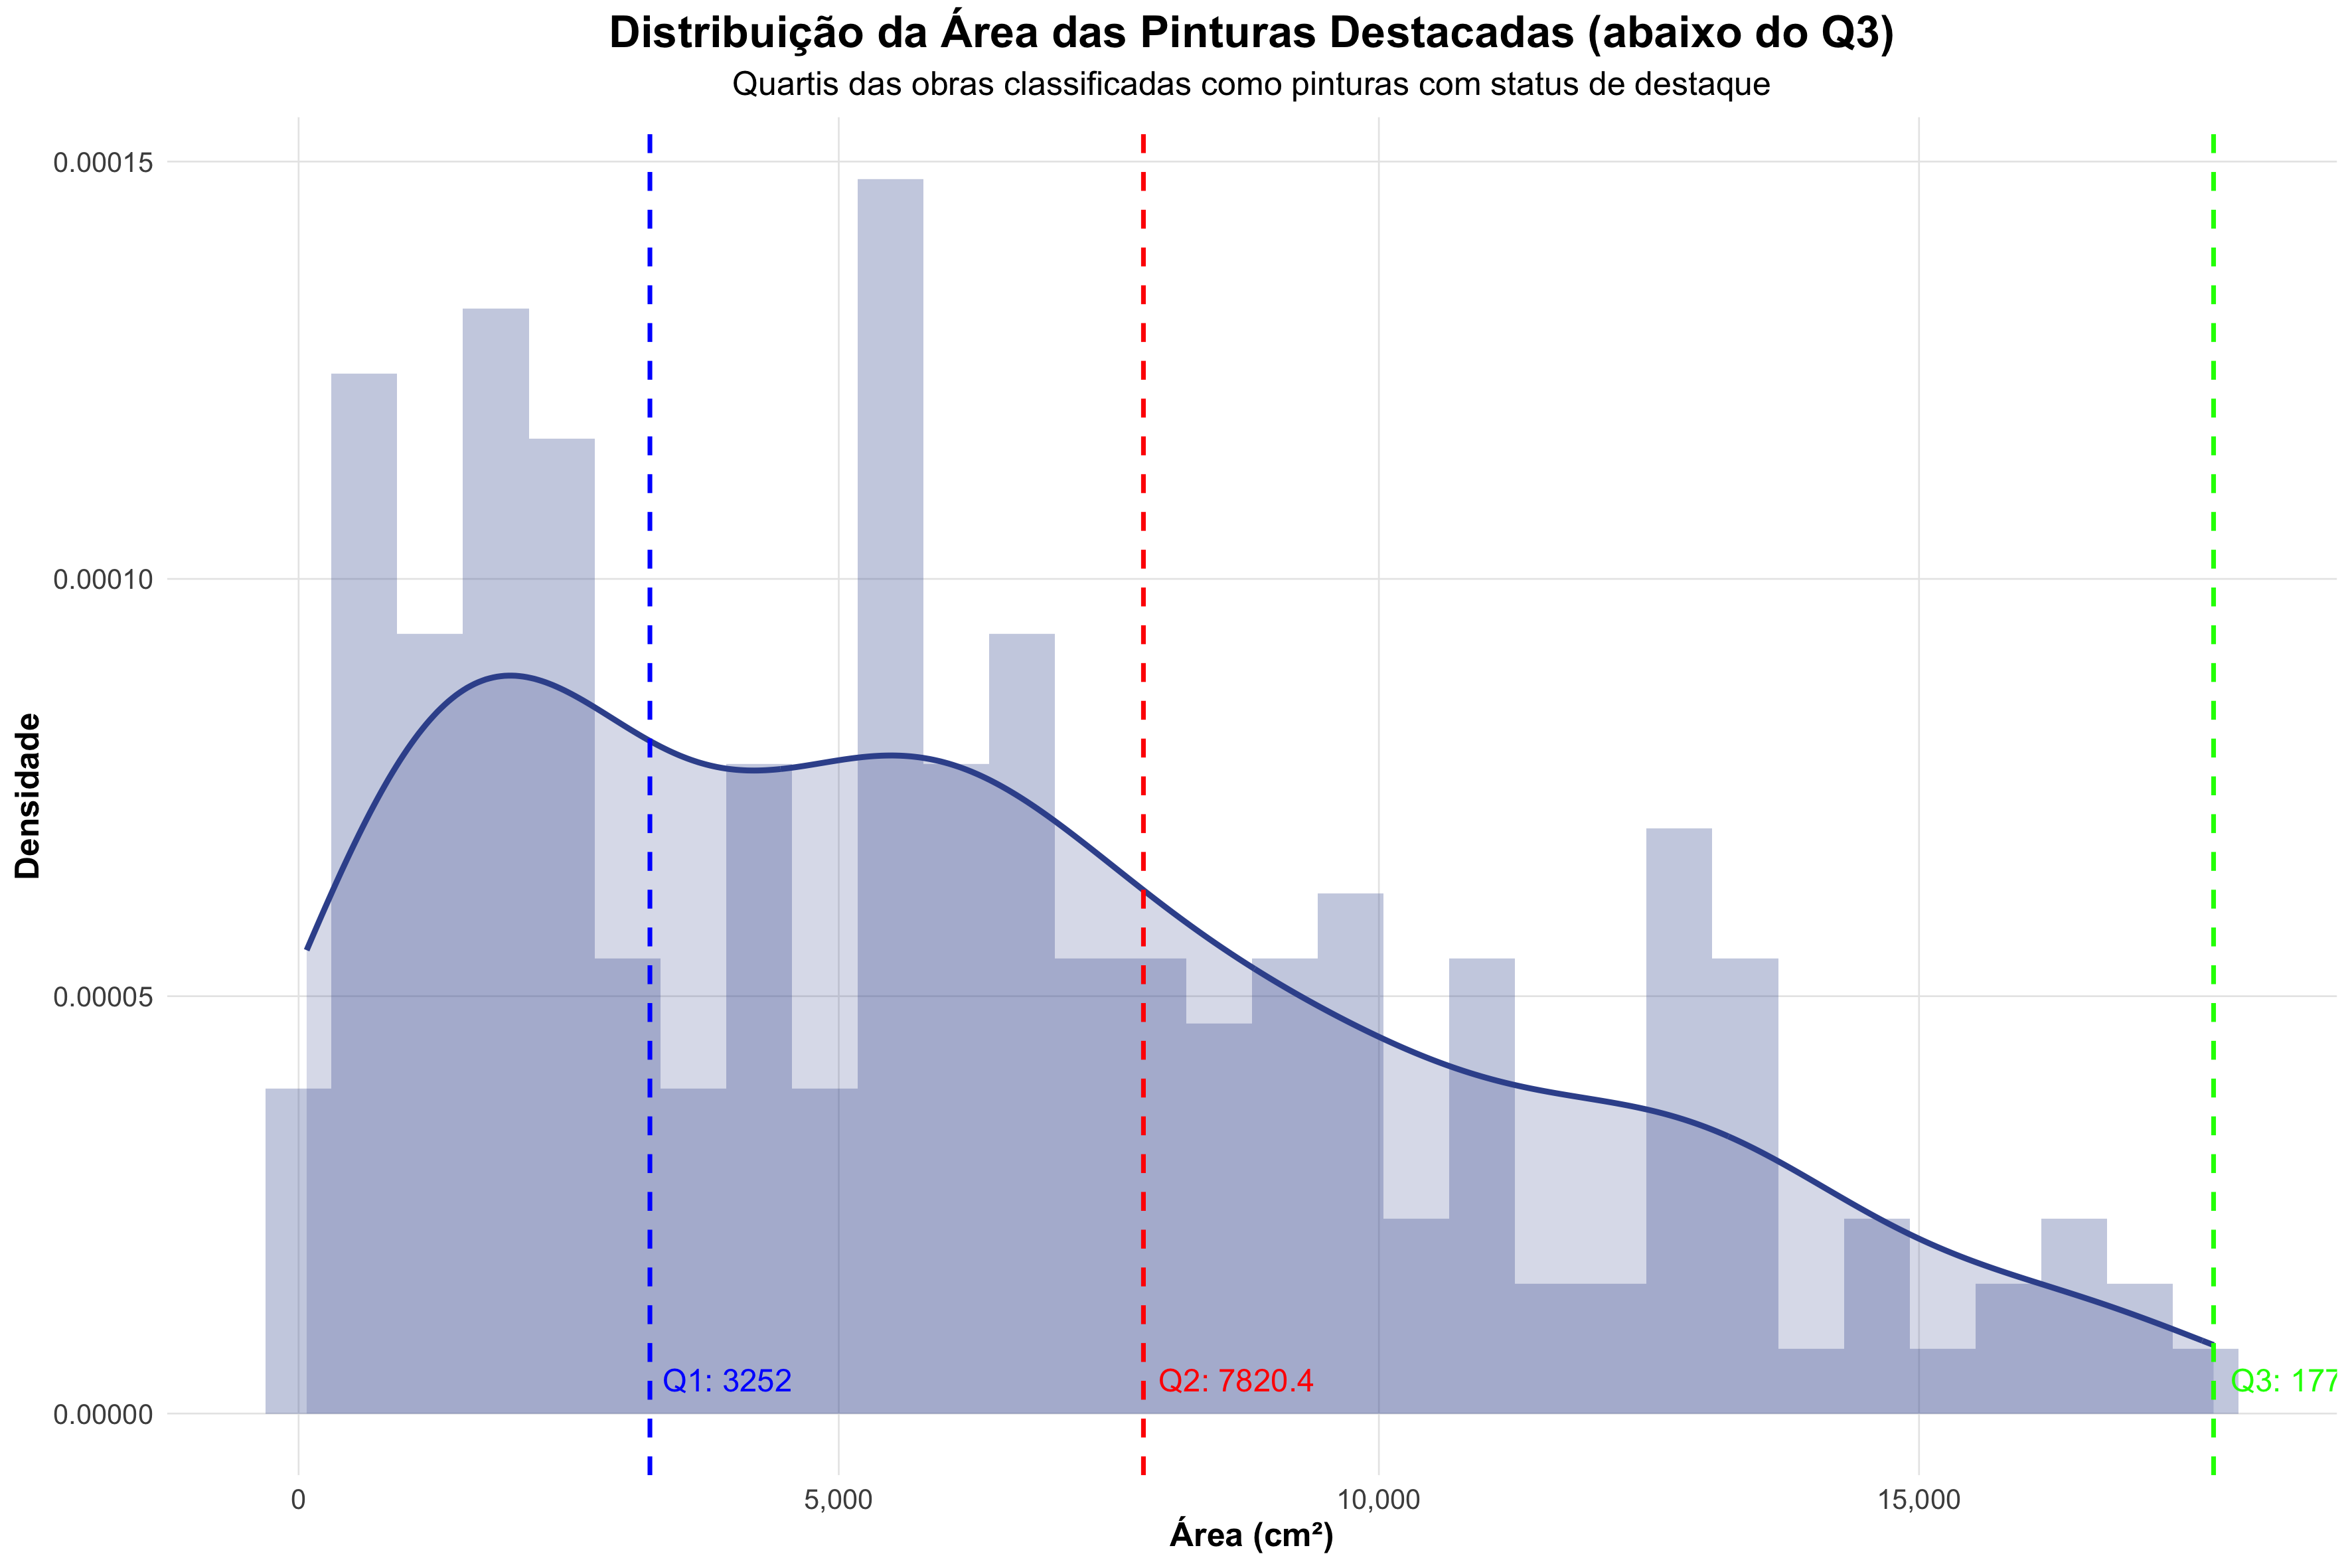
\includegraphics[width=\textwidth]{../imagens/densidade_pinturas_highlight_q3.png} 
        \caption{Densidade da Área das Pinturas em Destaque (abaixo do Q3).}
        \label{fig:densidade_pinturas_highlight}
    \end{subfigure}
    \caption{Distribuição de densidade das dimensões de obras em destaque (abaixo do Q3).}
    \label{fig:densidade_dimensoes_destaque}
\end{figure}

Ao observar esses dois gráficos (Figura~\ref{fig:densidade_dimensoes_destaque}), que mostram apenas as obras em destaque com dimensões abaixo do terceiro quartil, percebe-se que as obras mais valorizadas pela curadoria não são, em sua maioria, de grande porte. Isso sugere que, para uma obra ser considerada em destaque, não precisa apresentar grandes dimensões. Em outras palavras, é possível concluir que o tamanho não é a característica com maior peso na seleção curatorial. A popularidade de uma obra, portanto, parece estar mais relacionada a outros fatores, como a temática da obra.

\subsubsection{A Influência do Tempo na Popularidade}
Com a análise temporal das obras, observam-se padrões tanto na produção quanto na aquisição de esculturas e pinturas pelo Metropolitan Museum of Art. O gráfico a seguir mostra um aumento significativo na produção dessas obras a partir do século XIX, que se intensificou no século XX. Esse crescimento pode estar relacionado à expansão das escolas artísticas, à industrialização e até mesmo à maior disponibilidade de materiais e técnicas artísticas.

\begin{figure}[H]
    \centering
    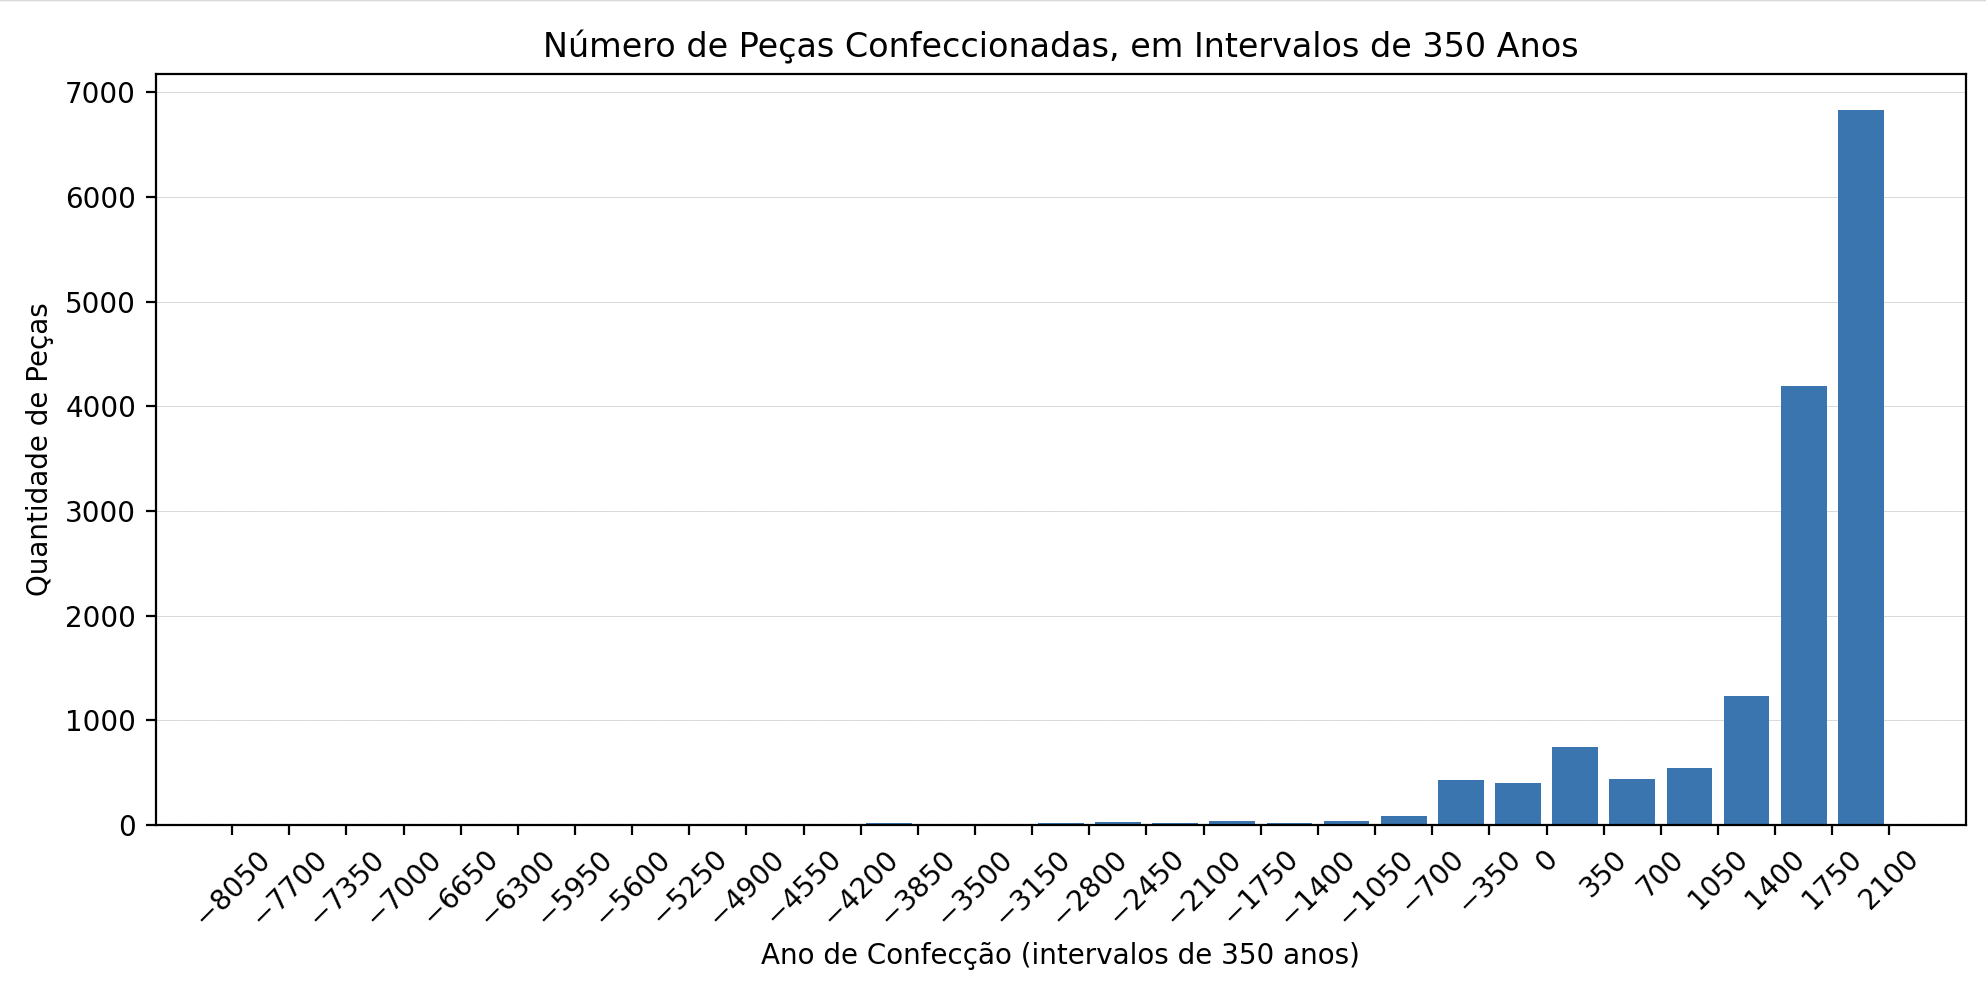
\includegraphics[width=0.6\textwidth]{../imagens/variaveis/ObjectBeginDate.png}
    \caption{Distribuição temporal da confecção das obras de pintura e escultura.}
    \label{fig:object_begin_date}
\end{figure}

Paralelamente, o gráfico de "Número de Peças Adquiridas por Intervalo de 5 Anos" mostra picos de aquisição pelo MET entre 1975 e 1990. Esse período, de fato, coincide com iniciativas do museu voltadas à diversificação e expansão de seu acervo \cite{metHistory}, incluindo a incorporação de coleções, como a do Museum of Primitive Art. Essa integração ampliou significativamente a representação de culturas não ocidentais no acervo do museu.

\begin{figure}[H]
    \centering
    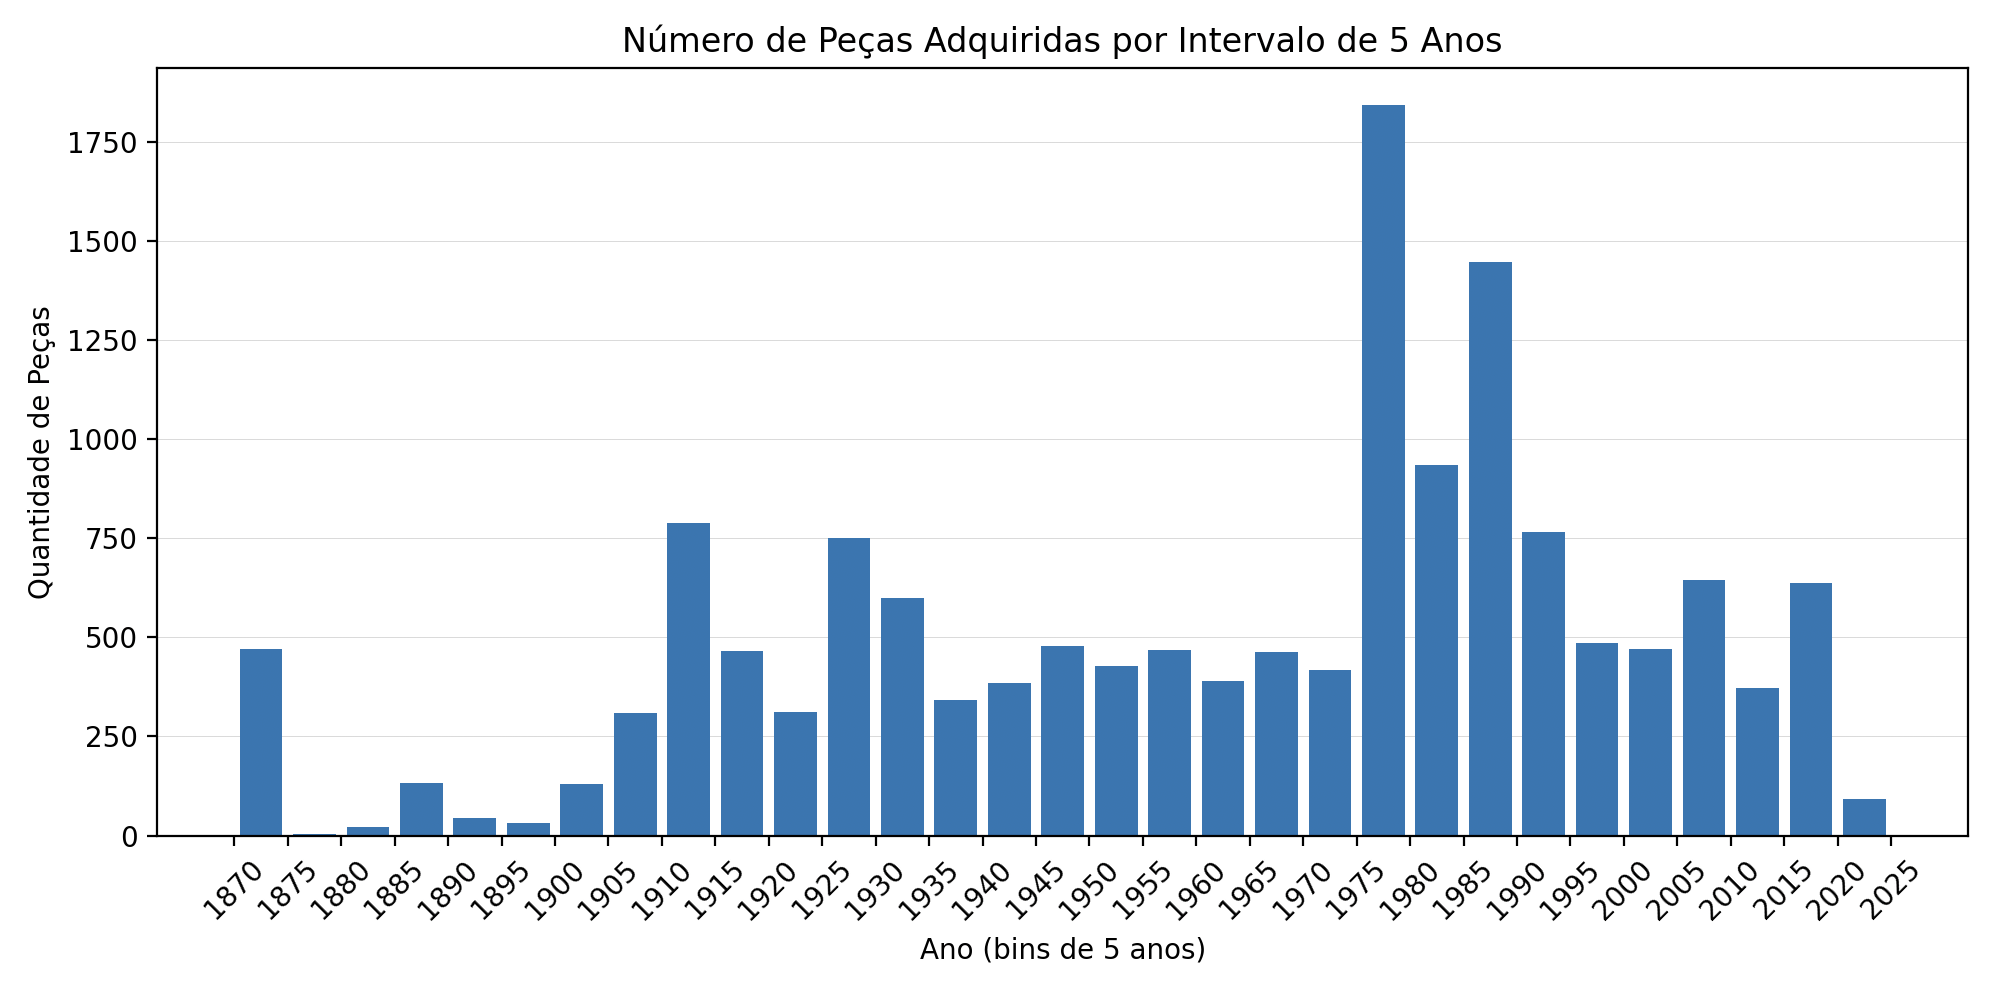
\includegraphics[width=0.8\textwidth]{../imagens/variaveis/AccessionYear.png}
    \caption{Número de peças adquiridas pelo MET por intervalo de 5 anos.}
    \label{fig:accession_year}
\end{figure}

Por fim, o gráfico a seguir destaca que as obras classificadas como "em destaque" tendem a ser mais recentes em comparação ao conjunto geral. Esse padrão pode estar relacionado à melhor conservação dessas peças, à sua relevância temática contemporânea ou, até, a uma curadoria que busca refletir valores e narrativas do presente. Esses dados reforçam a hipótese 2, sugerindo que a popularidade de uma obra, para o MET, está vinculada ao contexto socioeconômico e cultural de cada época.

\begin{figure}[H]
    \centering
    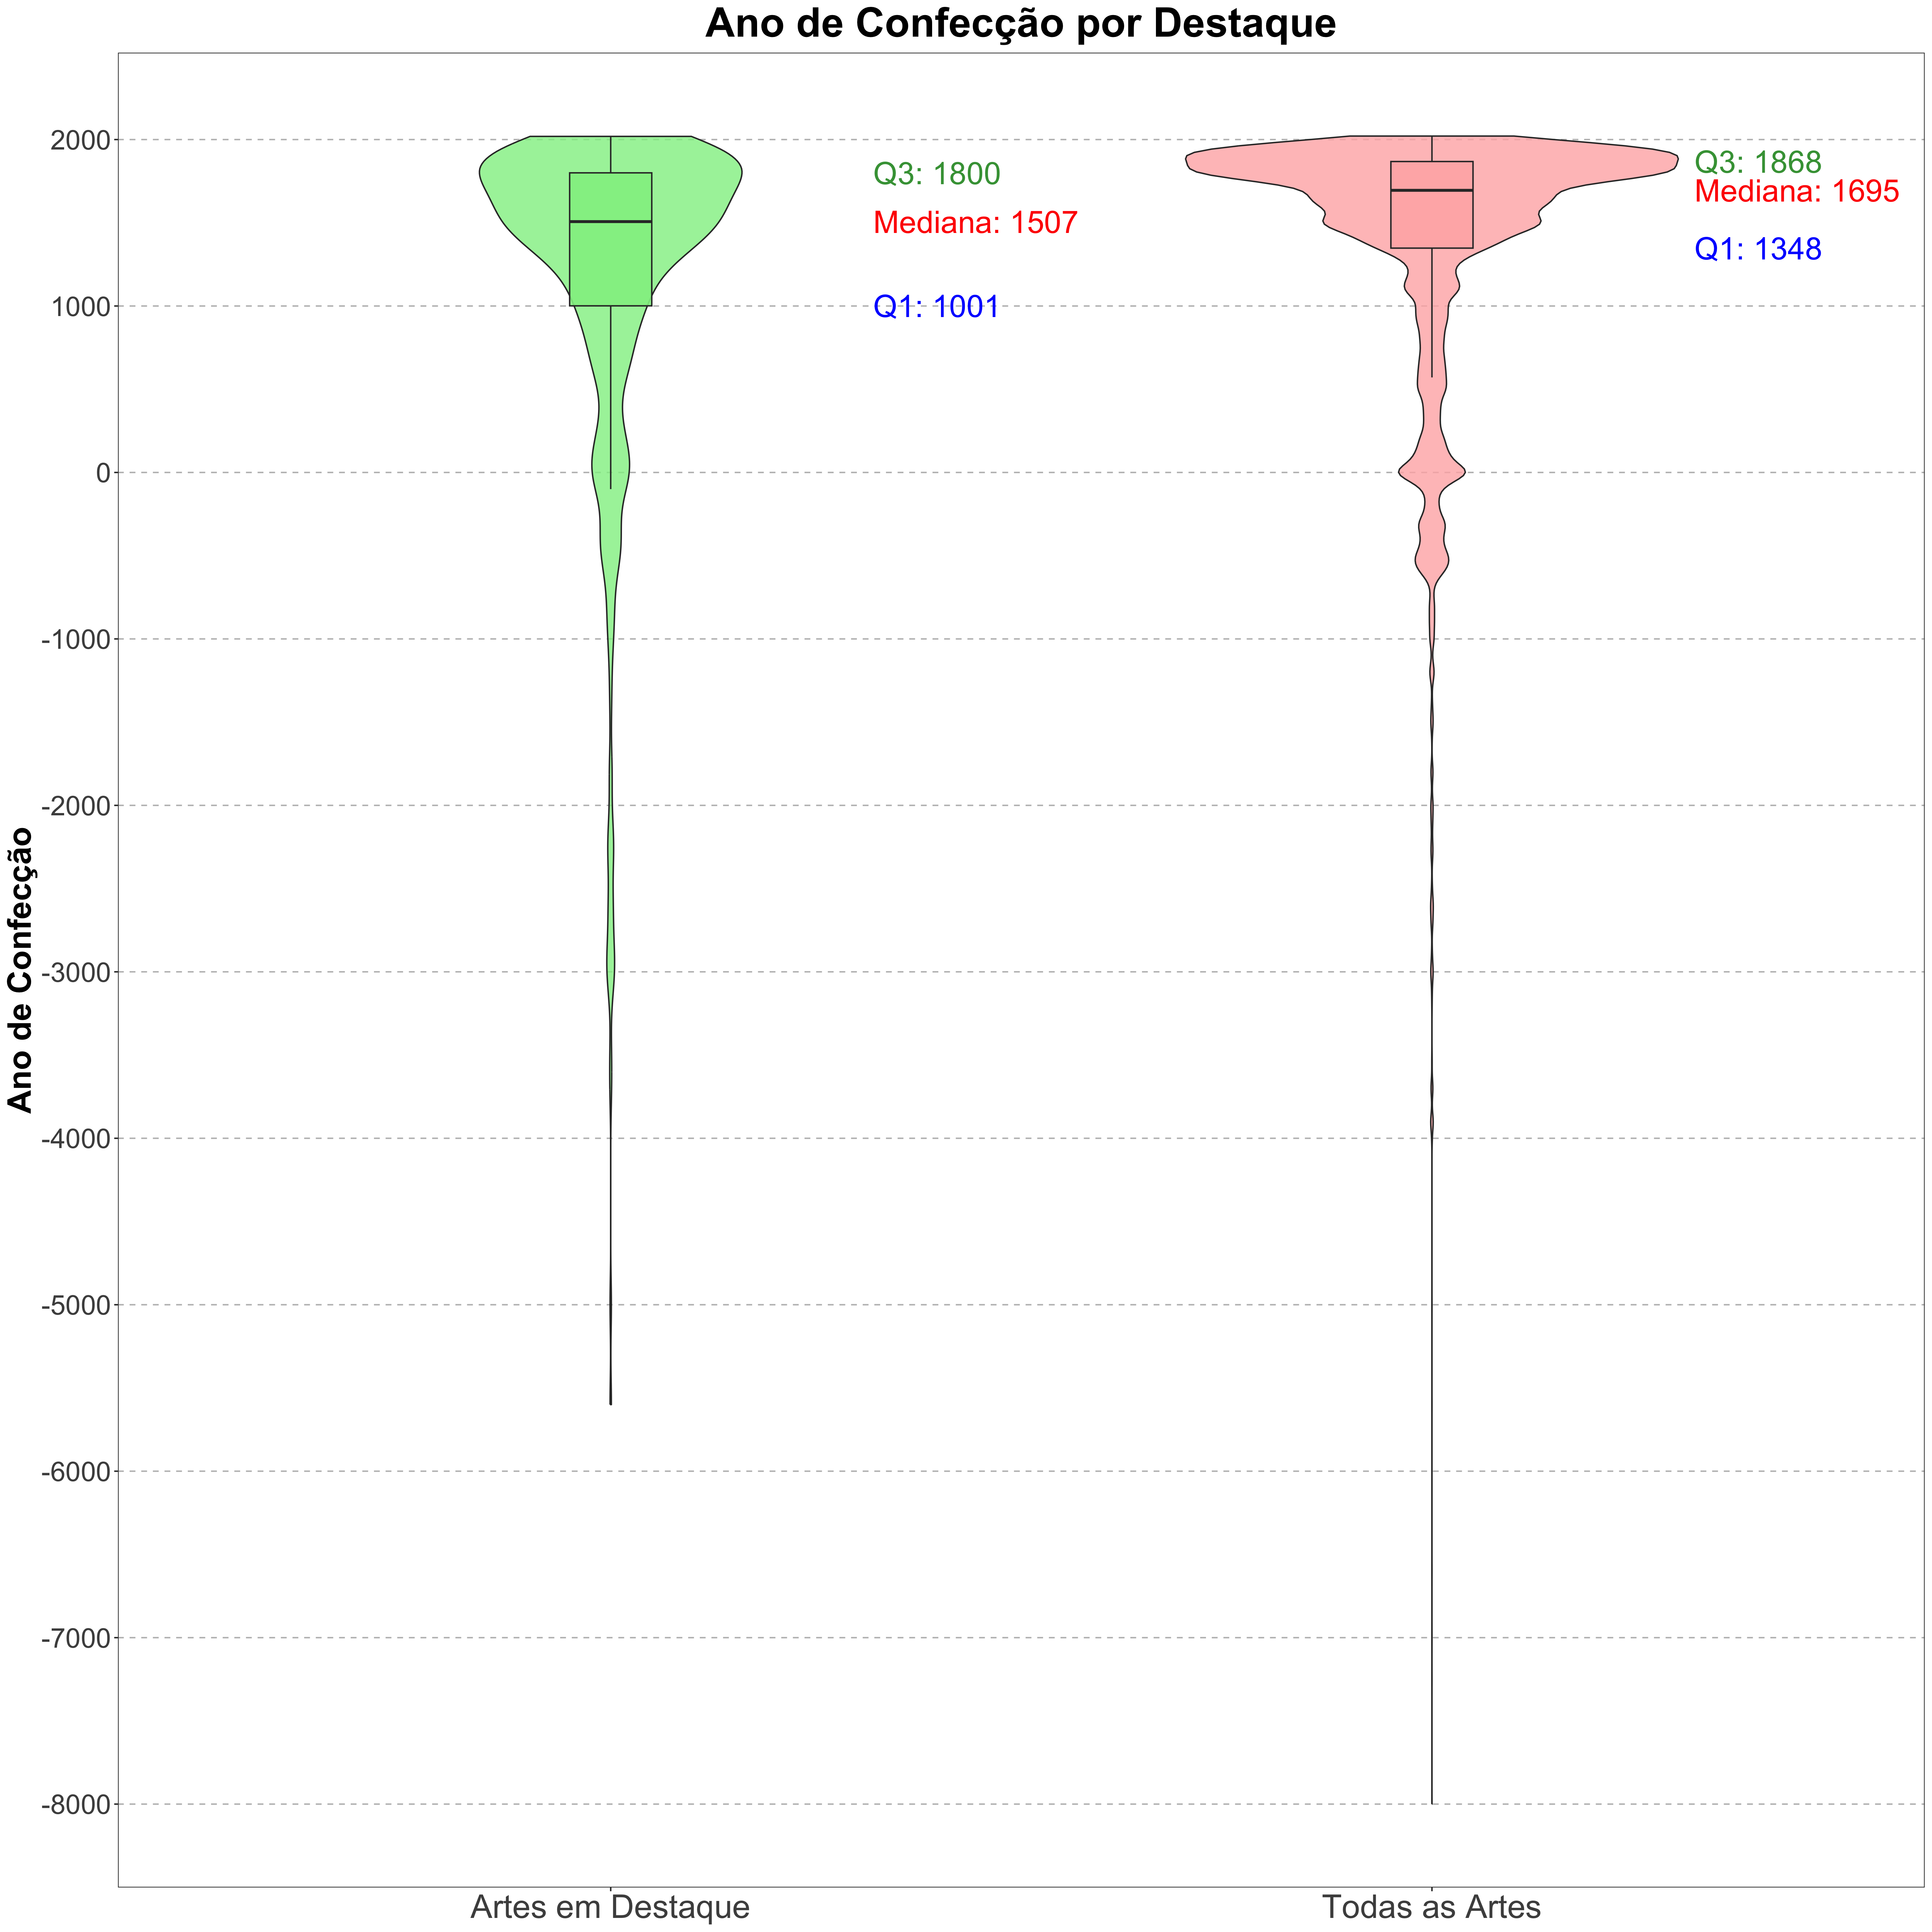
\includegraphics[width=0.55\textwidth]{../imagens/violin_plot_ano_destaque.png}
    \caption{Comparativo do ano de confecção entre obras em destaque e o acervo geral.}
    \label{fig:violin_ano_destaque}
\end{figure}

\subsection{Medidas de Resumo: Características Numéricas do Acervo}
Esta seção apresenta e discute as medidas de tendência central, dispersão e posição das principais variáveis numéricas do conjunto de dados analisado: ano de confecção, área das pinturas e volume das esculturas. O objetivo é oferecer uma visão quantitativa complementar aos gráficos já apresentados, mostrando a assimetria e a diversidade do acervo do Metropolitan Museum of Art.

\subsubsection{Ano de Confecção das Obras}
A variável que representa as datas de confecção das obras apresenta uma distribuição bastante ampla, com valores que variam de -8000 a 2021 (ano da última obra confeccionada). A média é de 1377,46, enquanto a mediana é de 1695, o que indica uma distribuição assimétrica à esquerda, o que é esperado considerando a pequena quantidade de obras extremamente antigas em comparação às contemporâneas. A maior densidade é observada no intervalo entre o primeiro e o terceiro quartil (Q1 = 1348; Q3 = 1868).

\begin{figure}[H]
    \centering
    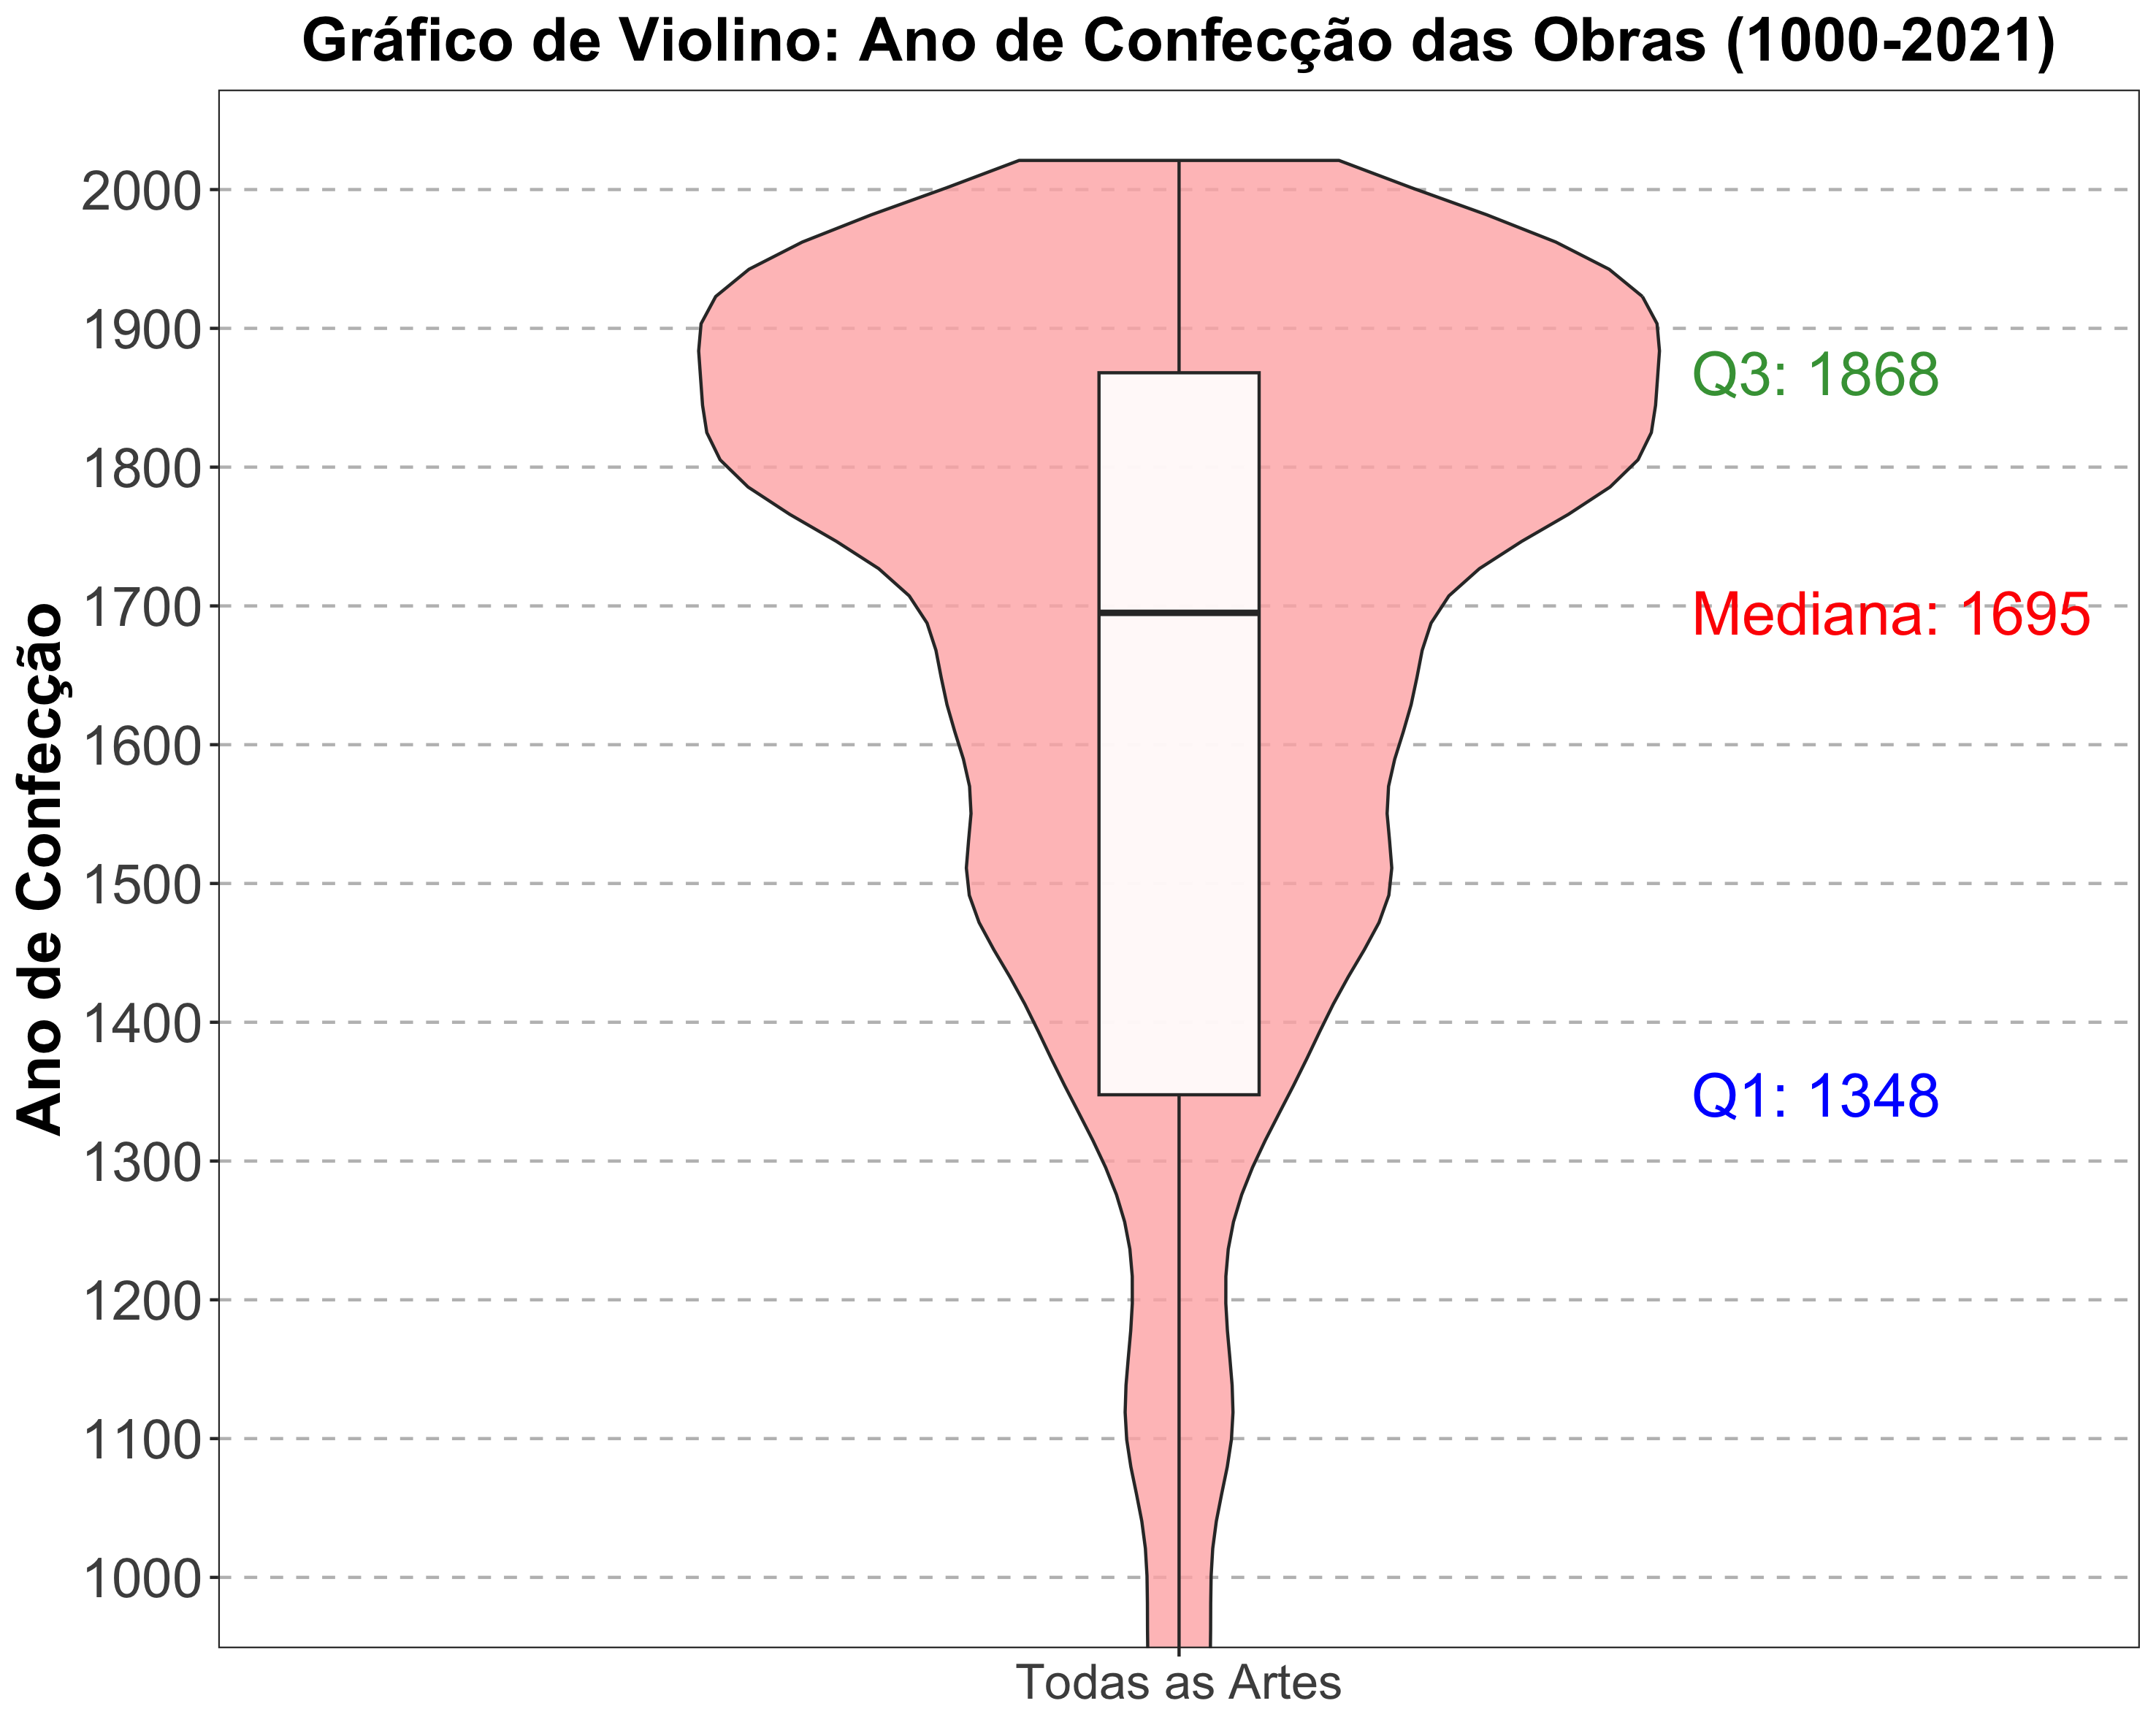
\includegraphics[width=0.6\textwidth]{../imagens/violin_plot_ano_todas_zoom.png}
    \caption{Distribuição do ano de confecção de todas as obras (com zoom entre 1000-2021).}
    \label{fig:violin_ano_todas_zoom}
\end{figure}

\subsubsection{Área das Pinturas}
A distribuição das áreas das pinturas varia desde valores mínimos muito pequenos (0,01 cm²) até mais de 443.000 cm². A média é de 6.718,47 cm², e o desvio padrão elevado (14.196,86 cm²) evidencia a alta dispersão e a presença de valores extremos. A mediana, entretanto, é de 2.036,25 cm², o que revela que a maior parte das obras possui dimensões mais modestas.

\subsubsection{Volume das Esculturas}
A variável do volume apresenta variações ainda mais acentuadas do que a da área, com valores que vão de 1,24 cm³ até mais de 51 milhões de cm³. A média é de 186.290,76 cm³, mas a mediana é de apenas 11.029,39 cm³ — mais uma vez revelando a forte assimetria da distribuição, com poucas esculturas de grande porte influenciando a média. Além disso, o elevado desvio padrão (mais de 1,5 milhão) e a variância muito alta (na escala de 10¹³) confirmam esse comportamento.

% Seção: Considerações Finais
\section{Considerações Finais}
Conforme os dados apresentados, nossas análises corroboram de modo consistente as hipóteses iniciais. A seguir, retomamos cada uma delas e destacamos as conclusões finais que emergem deste estudo.

\subsection*{Hipótese 1 - Material e território}
Observou-se que a escolha dos materiais nas obras de pintura e escultura está estreitamente ligada à disponibilidade regional. Exemplo disso é a prevalência de mármore em peças oriundas do Mediterrâneo e o uso de seda e papel em produções asiáticas. Adicionalmente, as técnicas desenvolvidas em cada cultura — adaptadas aos recursos locais — reforçam esse padrão, demonstrando que o "meio" (material) molda diretamente a expressão artística.

\subsection*{Hipótese 2 - Popularidade, temática e contexto temporal}
Constatou-se que o tamanho físico das obras pouco influencia sua classificação como destaque, ao passo que o conteúdo simbólico e histórico (temas humanos, religiosos, narrativas culturais) exerce papel determinante. Obras com forte carga narrativa são mais enfatizadas, o que reflete um viés antropocêntrico e humanitário na curadoria do MET. Além disso, peças mais recentes apresentam maior probabilidade de destaque, indicando preferência por temas contemporâneos e por práticas curatoriais atuais.

\subsection*{Limitações e Estudos Futuros}
A expressiva quantidade de registros sem atribuição de cultura limita a extensão das análises comparativas. Soma-se a isso o viés de aquisição do MET, que privilegia a arte europeia e norte-americana, reduzindo a representatividade de outras tradições. Para contornar essas restrições, recomenda-se, em estudos futuros, a inclusão de acervos de outros museus e a diversificação das categorias artísticas para além de pinturas e esculturas.

\subsection*{Síntese Final}
Em síntese, este trabalho reforça a ideia de que a arte funciona como um espelho do ambiente físico e social que a produz. Os resultados demonstram claramente a interdependência entre recursos territoriais, técnicas culturais e valores curatoriais. Para aprofundar essa compreensão, futuras pesquisas deverão explorar bases de dados internacionais e incorporar variáveis como a proveniência social dos autores e a dinâmica de circulação expositiva. Dessa forma, poderemos atingir uma visão mais abrangente sobre como território e tempo continuam a moldar a recepção e a memória das obras de arte.


\newpage
% Seção: Referências Bibliográficas
\section*{Referências Bibliográficas}
% Exemplo de referências no formato ABNT (ou o que for exigido)
\begin{thebibliography}{99}
  \bibitem{metOpenAccess} The Metropolitan Museum of Art Open Access CSV. Disponível em: \url{https://github.com/metmuseum/openaccess}
  \bibitem{metMakingTheMet} METROPOLITAN MUSEUM OF ART. Making the MET, 1870-2020. Disponível em: \url{https://www.metmuseum.org/exhibitions/listings/2020/making-the-met-1870-to-2020}
  \bibitem{metHistory} METROPOLITAN MUSEUM OF ART. History of the Museum. Disponível em: \url{https://www.metmuseum.org/about-the-met/history}
\end{thebibliography}

% Anexos (ex.: sintaxe utilizada, código R, etc.)
\appendix
\section{Anexos}

\subsection*{Código R: Gráfico de Densidade das Dimensões de Obras em Destaque}
\label{anx:codigo_histograma_dimensoes_highlight}
\begin{verbatim}
# carregando bibliotecas que vamos usar
library(ggplot2)
library(dplyr)
library(tidyr)
library(stringr)

# carregando o arquivo csv
df <- read.csv("trabalho1/tabela_met.csv", stringsAsFactors = FALSE, check.names = FALSE)

# renomeando as colunas para facilitar o uso no R
names(df)[names(df) == "Is Highlight"] <- "IsHighlight"
names(df)[names(df) == "Classification"] <- "Classificacao"

# convertendo IsHighlight para lógico
df$IsHighlight <- as.logical(df$IsHighlight)

# filtrando obras destacadas
obras_destacadas <- df %>%
  filter(IsHighlight == TRUE)

# filtrando pinturas e esculturas
pinturas <- obras_destacadas %>%
  filter(str_detect(tolower(Classificacao), "painting")) %>%
  filter(!is.na(area)) %>%
  # removendo outliers extremos para melhor visualização
  filter(area < quantile(area, 0.99, na.rm = TRUE))

esculturas <- obras_destacadas %>%
  filter(str_detect(tolower(Classificacao), "sculpture")) %>%
  filter(!is.na(volume)) %>%
  # removendo outliers extremos para melhor visualização
  filter(volume < quantile(volume, 0.99, na.rm = TRUE))

# calculando quartis para pinturas
q1_pintura <- quantile(pinturas$area, 0.25)
q2_pintura <- quantile(pinturas$area, 0.50) # mediana
q3_pintura <- quantile(pinturas$area, 0.75)

# calculando quartis para esculturas
q1_escultura <- quantile(esculturas$volume, 0.25)
q2_escultura <- quantile(esculturas$volume, 0.50) # mediana
q3_escultura <- quantile(esculturas$volume, 0.75)

# filtrando para mostrar apenas obras abaixo do q3
pinturas_abaixo_q3 <- pinturas %>% filter(area <= q3_pintura)
esculturas_abaixo_q3 <- esculturas %>% filter(volume <= q3_escultura)

# criando pasta para salvar imagens
dir.create("trabalho1/imagens", showWarnings = FALSE, recursive = TRUE)

# definindo cores e tema comum
cor_pintura <- "#3A539B"  # azul escuro
cor_escultura <- "#674172"  # roxo
tema_comum <- theme_minimal() +
  theme(
    plot.title = element_text(hjust = 0.5, size = 16, face = "bold"),
    plot.subtitle = element_text(hjust = 0.5, size = 12),
    axis.title = element_text(size = 12, face = "bold"),
    axis.text = element_text(size = 10),
    panel.grid.minor = element_blank(),
    panel.grid.major.x = element_line(color = "#E8E8E8", size = 0.3),
    panel.grid.major.y = element_line(color = "#E8E8E8", size = 0.3),
    legend.position = "none"
  )

# preparando dataframes para anotações de quartis
quartis_pintura <- data.frame(
  quartil = c("Q1", "Q2", "Q3"),
  valor = c(q1_pintura, q2_pintura, q3_pintura),
  cor = c("blue", "red", "green")
)

quartis_escultura <- data.frame(
  quartil = c("Q1", "Q2", "Q3"),
  valor = c(q1_escultura, q2_escultura, q3_escultura),
  cor = c("blue", "red", "green")
)

# gráfico de densidade para pinturas (área) abaixo do Q3
densidade_pinturas <- ggplot(pinturas_abaixo_q3, aes(x = area)) +
  # histograma semi-transparente por baixo
  geom_histogram(aes(y = after_stat(density)), fill = cor_pintura, alpha = 0.3, bins = 30) +
  # linha de densidade suavizada
  geom_density(color = cor_pintura, linewidth = 1, fill = cor_pintura, alpha = 0.2) +
  # adicionando linhas verticais dos quartis
  geom_vline(data = quartis_pintura, aes(xintercept = valor, color = quartil), 
             linetype = "dashed", linewidth = 0.8) +
  # anotações dos quartis
  geom_text(data = quartis_pintura,
            aes(x = valor, y = 0, label = paste0(quartil, ": ", round(valor, 1)), color = quartil),
            hjust = -0.1, vjust = -1, size = 4) +
  # definindo cores para os quartis
  scale_color_manual(values = c("Q1" = "blue", "Q2" = "red", "Q3" = "green")) +
  # ajustando eixos e títulos
  scale_x_continuous(labels = scales::comma) +
  labs(
    title = "Distribuição da Área das Pinturas Destacadas (abaixo do Q3)",
    subtitle = "Quartis das obras classificadas como pinturas com status de destaque",
    x = "Área (cm²)",
    y = "Densidade"
  ) +
  tema_comum

# gráfico de densidade para esculturas (volume) abaixo do Q3
densidade_esculturas <- ggplot(esculturas_abaixo_q3, aes(x = volume)) +
  # histograma semi-transparente por baixo
  geom_histogram(aes(y = after_stat(density)), fill = cor_escultura, alpha = 0.3, bins = 30) +
  # linha de densidade suavizada
  geom_density(color = cor_escultura, linewidth = 1, fill = cor_escultura, alpha = 0.2) +
  # adicionando linhas verticais dos quartis
  geom_vline(data = quartis_escultura, aes(xintercept = valor, color = quartil), 
             linetype = "dashed", linewidth = 0.8) +
  # anotações dos quartis
  geom_text(data = quartis_escultura,
            aes(x = valor, y = 0, label = paste0(quartil, ": ", round(valor, 1)), color = quartil),
            hjust = -0.1, vjust = -1, size = 4) +
  # definindo cores para os quartis
  scale_color_manual(values = c("Q1" = "blue", "Q2" = "red", "Q3" = "green")) +
  # ajustando eixos e títulos
  scale_x_continuous(labels = scales::comma) +
  labs(
    title = "Distribuição do Volume das Esculturas Destacadas (abaixo do Q3)",
    subtitle = "Quartis das obras classificadas como esculturas com status de destaque",
    x = "Volume (cm³)",
    y = "Densidade"
  ) +
  tema_comum

# exibindo os gráficos
print(densidade_pinturas)
print(densidade_esculturas)

# salvando os gráficos
ggsave(
  filename = "trabalho1/imagens/densidade_pinturas_highlight_q3.png",
  plot = densidade_pinturas,
  width = 30,
  height = 20,
  dpi = 300,
  units = "cm",
  bg = "white"
)

ggsave(
  filename = "trabalho1/imagens/densidade_esculturas_highlight_q3.png",
  plot = densidade_esculturas,
  width = 30,
  height = 20,
  dpi = 300,
  units = "cm",
  bg = "white"
) 
\end{verbatim}

\subsection*{Código R: Gráfico de Pareto das Tags das Obras em Destaque}
\label{anx:codigo_pareto_tags_highlight}
\begin{verbatim}
# carregando bibliotecas que vamos usar
library(ggplot2)
library(dplyr)
library(tidyr)
library(stringr)
library(forcats)

# carregando o arquivo csv
df <- read.csv("trabalho1/tabela_met.csv", stringsAsFactors = FALSE, check.names = FALSE)

# renomeando as colunas
names(df)[names(df) == "Tags"] <- "Tags"
names(df)[names(df) == "Is Highlight"] <- "IsHighlight"

# convertendo IsHighlight para lógico
df$IsHighlight <- as.logical(df$IsHighlight)

# separando as tags (apenas para obras em destaque)
tags_destaque <- df %>%
  filter(!is.na(Tags) & Tags != "" & IsHighlight == TRUE) %>%
  select(Tags) %>%
  # separando as tags pelo delimitador "|"
  mutate(Tags = strsplit(Tags, "\\|")) %>%
  # expandindo a lista de tags para ter uma linha por tag
  unnest(Tags) %>%
  # limpando espaços extras
  mutate(Tags = trimws(Tags))

# contando as tags em destaque mais frequentes
top_tags_destaque <- tags_destaque %>%
  count(Tags, sort = TRUE) %>%
  slice_head(n = 10)

# preparando os dados para o gráfico de pareto
dados_pareto <- top_tags_destaque %>%
  # adicionando a categoria "Outros" para as tags menos frequentes
  bind_rows(
    tags_destaque %>%
      anti_join(top_tags_destaque, by = "Tags") %>%
      count(name = "n") %>%
      mutate(Tags = "Outros")
  ) %>%
  # ordenando do maior para o menor, com "Outros" no final
  arrange(desc(n)) %>%
  mutate(
    # Criando fator para manter a ordem no gráfico
    Tags = factor(Tags, levels = c(pull(top_tags_destaque, Tags), "Outros")),
    # Calculando a porcentagem
    porcentagem = n / sum(n) * 100,
    # Calculando a porcentagem acumulada
    porcentagem_acumulada = cumsum(porcentagem),
    # Adicionando rótulos para o gráfico
    rotulo_valor = n,
    rotulo_porcentagem = paste0(round(porcentagem), "%")
  )

# definindo cores
cor_barras <- "#5D8AA8"
cor_linha_pareto <- "#7B3F00"

# criando o gráfico de pareto
grafico_pareto <- ggplot() +
  # adicionando as barras
  geom_bar(
    data = dados_pareto,
    aes(x = Tags, y = n, fill = "Contagem"),
    stat = "identity",
    width = 0.7
  ) +
  # adicionando a linha de porcentagem acumulada
  geom_line(
    data = dados_pareto,
    aes(x = Tags, y = porcentagem_acumulada * max(n) / 100, group = 1, color = "% Acumulada"),
    size = 0.8
  ) +
  # adicionando pontos à linha de porcentagem acumulada
  geom_point(
    data = dados_pareto,
    aes(x = Tags, y = porcentagem_acumulada * max(n) / 100, group = 1, color = "% Acumulada"),
    size = 2.5,
    shape = 21,
    fill = "white",
    stroke = 0.8
  ) +
  # adicionando rótulos de porcentagem acumulada
  geom_text(
    data = dados_pareto,
    aes(x = Tags, y = porcentagem_acumulada * max(n) / 100, 
        label = paste0(round(porcentagem_acumulada), "%")),
    vjust = -0.8,
    color = cor_linha_pareto,
    fontface = "bold",
    size = 3.2
  ) +
  # adicionando rótulos de contagem em cada barra
  geom_text(
    data = dados_pareto,
    aes(x = Tags, y = n / 2, label = rotulo_valor),
    color = "white",
    fontface = "bold",
    size = 3.2
  ) +
  # configurando os eixos
  scale_y_continuous(
    name = "Contagem",
    sec.axis = sec_axis(~ . * 100 / max(dados_pareto$n), name = "% Acumulada")
  ) +
  # definindo cores
  scale_fill_manual(values = c("Contagem" = cor_barras)) +
  scale_color_manual(values = c("% Acumulada" = cor_linha_pareto)) +
  # personalizando o tema
  theme_minimal(base_size = 12) +
  theme(
    plot.title = element_text(hjust = 0.5, size = 16, face = "bold", margin = margin(b = 10)),
    plot.subtitle = element_text(hjust = 0.5, size = 12, margin = margin(b = 20)),
    axis.title.x = element_blank(),
    axis.title.y = element_text(size = 12, face = "bold"),
    axis.text.x = element_text(angle = 45, hjust = 1, size = 10),
    axis.text.y = element_text(size = 10),
    legend.title = element_blank(),
    legend.position = "top",
    legend.margin = margin(b = 10),
    panel.grid.minor = element_blank(),
    panel.grid.major.x = element_blank(),
    panel.grid.major.y = element_line(color = "#E8E8E8", size = 0.3),
    panel.background = element_rect(fill = "white", color = NA),
    plot.background = element_rect(fill = "white", color = NA),
    plot.margin = margin(t = 20, r = 20, b = 20, l = 20)
  ) +
  # adicionando título e subtítulo
  labs(
    title = "Top 10 tags em obras destacadas",
    subtitle = "Distribuição das tags mais frequentes em obras com destaque"
  )

# exibindo o gráfico
print(grafico_pareto)

# criando diretório para salvar a imagem se não existir
dir.create("trabalho1/imagens", showWarnings = FALSE, recursive = TRUE)

# salvando o gráfico
ggsave(
  filename = "trabalho1/imagens/pareto_tags_highlight.png",
  plot = grafico_pareto,
  width = 30,
  height = 20,
  dpi = 300,
  units = "cm",
  bg = "white"
) 
\end{verbatim}

\subsection*{Código R: Gráfico de Pizza da Análise de Materiais por Cultura}
\label{anx:codigo_piechart_cultura_material}
\begin{verbatim}
# carregando bibliotecas que vamos usar
library(ggplot2)
library(dplyr)
library(tidyr)
library(forcats) # para fct_reorder

# carregando o arquivo csv
df <- read.csv("trabalho1/tabela_met.csv", stringsAsFactors = FALSE, check.names = FALSE)

# renomeando as colunas
names(df)[names(df) == "Culture"] <- "Cultura"
names(df)[names(df) == "Medium"] <- "Meio"

# encontrando as 5 culturas mais frequentes
top5_culturas <- df %>%
  filter(Cultura != "" & !is.na(Cultura)) %>%
  count(Cultura, sort = TRUE) %>%
  slice_head(n = 5) %>%
  pull(Cultura)

# processando dados para os pie charts
df_piechart_data <- df %>%
  filter(Cultura %in% top5_culturas & Meio != "" & !is.na(Meio)) %>%
  count(Cultura, Meio) %>%
  group_by(Cultura) %>%
  mutate(
    rank = dense_rank(desc(n)), # rank para pegar os top 5 meios
    Meio_grupo = ifelse(rank <= 5, Meio, "Outros"),
    Meio_grupo = factor(Meio_grupo) # convertendo para fator
  ) %>%
  group_by(Cultura, Meio_grupo) %>%
  summarise(contagem = sum(n), .groups = 'drop') %>%
  group_by(Cultura) %>%
  mutate(
    porcentagem = round(contagem / sum(contagem) * 100, 1),
    Meio_grupo = fct_reorder(Meio_grupo, porcentagem, .desc = TRUE)
  ) %>%
  # ordenando os dados para que as fatias do piechart também sigam a ordem da legenda
  arrange(Cultura, desc(porcentagem))

# criando diretorio para salvar as imagens
dir.create("trabalho1/imagens/piecharts_culturas", showWarnings = FALSE, recursive = TRUE)

# definindo cores
cores_piechart <- c("#377EB8", "#4DAF4A", "#E41A1C", "#984EA3", "#FF7F00", "#A65628", "#F781BF", "#F1C232") # Adicionada mais uma cor caso 'Outros' seja frequente

# gerando um piechart para cada cultura
for (cult_idx in seq_along(top5_culturas)) {
  cultura_atual <- top5_culturas[cult_idx]
  
  dados_cultura_atual <- df_piechart_data %>%
    filter(Cultura == cultura_atual)
  
  # criando o piechart
  grafico <- ggplot(dados_cultura_atual, 
                    aes(x = "", y = porcentagem, fill = Meio_grupo)) +
    geom_bar(stat = "identity", width = 1, color = "white", linewidth = 0.6) +
    coord_polar("y", start = 0) +
    geom_text(
      aes(label = ifelse(porcentagem > 3, paste0(porcentagem, "%"), "")),
      position = position_stack(vjust = 0.5),
      color = "white",
      fontface = "bold",
      size = 4.5
    ) +
    scale_fill_manual(values = cores_piechart) +
    labs(
      title = paste("Cultura:", cultura_atual),
      subtitle = "Distribuição dos materiais",
      fill = "Material"
    ) +
    theme_bw(
      base_size = 14 # tamanho base da fonte para o tema
    ) +
    theme(
      plot.title = element_text(hjust = 0.5, size = 18, face = "bold"),
      plot.subtitle = element_text(hjust = 0.5, size = 14, margin = margin(b = 15)),
      legend.position = "bottom",
      legend.title = element_text(size = 12, face = "bold"),
      legend.text = element_text(size = 10),
      legend.key.size = unit(0.7, "cm"),
      panel.grid = element_blank(),
      axis.text = element_blank(),
      axis.ticks = element_blank(),
      axis.title = element_blank(),
      panel.border = element_blank(), 
      plot.background = element_rect(fill = "white", colour = "white"),
      plot.margin = margin(1, 1, 1, 1, "cm") # adicionando margem ao redor do grafico
    )
  
  # nome do arquivo para salvar
  nome_arquivo <- paste0("trabalho1/imagens/piecharts_culturas/piechart_", 
                         gsub("[^a-zA-Z0-9_]", "_", tolower(cultura_atual)), ".png")
  
  # salvando a visualizacao individual
  ggsave(
    filename = nome_arquivo,
    plot = grafico,
    width = 30,
    height = 20,
    dpi = 300,
    units = "cm",
    bg = "white"
  )
} 
\end{verbatim}

\subsection*{Código R: Gráfico de Violino das Obras em Destaque por Ano}
\label{anx:codigo_violin_plot_year}
\begin{verbatim}

# carregando bibliotecas que vamos usar
library(ggplot2)
library(dplyr)
library(tidyr)

# carregando o arquivo csv
df <- read.csv("trabalho1/tabela_met.csv", stringsAsFactors = FALSE, check.names = FALSE)

# renomeando as colunas para facilitar o uso no R
names(df)[names(df) == "Is Highlight"] <- "IsHighlight"
names(df)[names(df) == "Object Begin Date"] <- "ObjectBeginDate"

# mudando o tipo das colunas para facilitar o uso
df$ObjectBeginDate <- as.numeric(df$ObjectBeginDate) # numero
df$IsHighlight <- as.logical(df$IsHighlight)       # verdadeiro ou falso

# ----

# criando um dataframe para o grupo de destaques
destaques_plot_data <- data.frame(
  Ano = df$ObjectBeginDate[df$IsHighlight == TRUE],
  Grupo = "Artes em Destaque"
)

# criando um dataframe para o grupo de todas as artes
todas_plot_data <- data.frame(
  Ano = df$ObjectBeginDate,
  Grupo = "Todas as Artes"
)

# juntando os dois dataframes em um só para usar no grafico
plot_df <- rbind(destaques_plot_data, todas_plot_data)

# nomeando os grupos
plot_df$Grupo <- factor(plot_df$Grupo, levels = c("Artes em Destaque", "Todas as Artes"))

# ----

# calculando as estatisticas para as anotações
stats_summary <- plot_df %>%
  group_by(Grupo) %>%
  summarise(
    q1 = quantile(Ano, 0.25, na.rm = TRUE),
    mediana = median(Ano, na.rm = TRUE),
    q3 = quantile(Ano, 0.75, na.rm = TRUE),
    .groups = 'drop' 
  )

# dataframe responsavel por colocar as anotações no grafico
annotations_df <- stats_summary %>%
  pivot_longer(
    cols = c(q1, mediana, q3),
    names_to = "stat_type",
    values_to = "y_pos"
  ) %>%
  mutate(
    label_prefix = case_when(
      stat_type == "q1" ~ "Q1:",
      stat_type == "mediana" ~ "Mediana:",
      stat_type == "q3" ~ "Q3:",
      TRUE ~ stat_type
    ),
    label = paste(label_prefix, round(y_pos)),
    text_color = case_when(
      stat_type == "q1" ~ "blue",
      stat_type == "mediana" ~ "red",
      stat_type == "q3" ~ "#439F43FF",
      TRUE ~ "black"
    )
  )

# ----

violin_plot_ano_destaque <- ggplot(plot_df, aes(x = Grupo, y = Ano, fill = Grupo)) + # criando o grafico
  geom_violin(width = 0.6, alpha = 0.8, show.legend = FALSE) + # violino
  geom_boxplot(width = 0.1, outlier.shape = NA, alpha = 0.9, show.legend = FALSE) + # caixa dentro do violino
  scale_fill_manual(values = c("Artes em Destaque" = "#90ee90", "Todas as Artes" = "#ffb3b3")) + # cores
  geom_text(
    data = annotations_df,
    aes(x = Grupo, y = y_pos, label = label, color = text_color),
    nudge_x = 0.32,
    size = 8,
    hjust = 0
  ) +
  scale_color_identity() +
  labs(
    title = "Ano de Confecção por Destaque",
    x = NULL,
    y = "Ano de Confecção"
  ) +
  
  # ajusta as legendas do eixo y
  scale_y_continuous(breaks = scales::pretty_breaks(n = 15)) +
  theme_bw() + 
  # coisas do tema
  theme(
    panel.grid.major.y = element_line(color = "grey", linetype = "dashed"), 
    panel.grid.minor.y = element_blank(), 
    panel.grid.major.x = element_blank(),
    plot.title = element_text(hjust = 0.5, size = 30, face = "bold"), 
    axis.title.x = element_text(size = 20, face = "bold"),
    axis.title.y = element_text(size = 24, face = "bold"),
    axis.text.x = element_text(size = 24),
    axis.text.y = element_text(size = 20)
  )

# ----

# exibe o grafico
print(violin_plot_ano_destaque)

# salva o grafico como arquivo
ggsave(
  filename = "trabalho1/imagens/violin_plot_ano_destaque.png",
  plot = violin_plot_ano_destaque,
  width = 50,
  height = 50,
  dpi = 300,
  units = "cm"
) 

# ---- INÍCIO: NOVO GRÁFICO APENAS 'TODAS AS ARTES' COM ZOOM ----

# criando um dataframe apenas para o grupo 'todas as artes'
# reutilizando 'todas_plot_data' já criado anteriormente no script
plot_df_todas <- todas_plot_data

# garantindo que 'grupo' seja um fator (embora aqui seja apenas um nível)
# isso ajuda o ggplot a tratar o eixo x corretamente
plot_df_todas$Grupo <- factor(plot_df_todas$Grupo)

# calculando as estatisticas para as anotações para 'todas as artes'
stats_summary_todas <- plot_df_todas %>%
  group_by(Grupo) %>% # 'Grupo' aqui será sempre 'Todas as Artes'
  summarise(
    q1 = quantile(Ano, 0.25, na.rm = TRUE),
    mediana = median(Ano, na.rm = TRUE),
    q3 = quantile(Ano, 0.75, na.rm = TRUE),
    .groups = 'drop' 
  )

# dataframe responsavel por colocar as anotações no grafico para 'todas as artes'
annotations_df_todas <- stats_summary_todas %>%
  pivot_longer(
    cols = c(q1, mediana, q3),
    names_to = "stat_type",
    values_to = "y_pos"
  ) %>%
  mutate(
    label_prefix = case_when(
      stat_type == "q1" ~ "Q1:",
      stat_type == "mediana" ~ "Mediana:",
      stat_type == "q3" ~ "Q3:",
      TRUE ~ stat_type # caso improvável de outros tipos de estatística
    ),
    label = paste(label_prefix, round(y_pos)),
    # definindo cores para as anotações de q1, mediana e q3
    text_color = case_when(
      stat_type == "q1" ~ "blue",
      stat_type == "mediana" ~ "red",
      stat_type == "q3" ~ "#439F43FF", # verde escuro
      TRUE ~ "black" # cor padrão para outros casos
    )
  )

# criando o gráfico de violino para 'todas as artes' com zoom
violin_plot_ano_todas_zoom <- ggplot(plot_df_todas, aes(x = Grupo, y = Ano)) + 
  geom_violin(fill = "#ffb3b3", width = 0.6, alpha = 0.8, show.legend = FALSE) + # usando a cor de 'todas as artes'
  geom_boxplot(width = 0.1, outlier.shape = NA, alpha = 0.9, show.legend = FALSE) + # caixa dentro do violino
  geom_text(
    data = annotations_df_todas,
    aes(x = Grupo, y = y_pos, label = label, color = text_color),
    nudge_x = 0.32, # ajustando a posição horizontal do texto
    size = 7,       # tamanho do texto das anotações
    hjust = 0       # alinhamento horizontal
  ) +
  scale_color_identity() + # aplicando as cores definidas em 'text_color'
  coord_cartesian(ylim = c(1000, 2022)) + # aplicando zoom no eixo y sem remover dados
  labs(
    title = "Gráfico de Violino: Ano de Confecção das Obras (1000-2022)",
    x = NULL, # removendo o rótulo do eixo x pois há apenas um grupo
    y = "Ano de Confecção"
  ) +
  scale_y_continuous(breaks = scales::pretty_breaks(n = 12)) + # ajustando os breaks para o novo intervalo do eixo y
  theme_bw() + 
  # aplicando tema similar ao gráfico original
  theme(
    panel.grid.major.y = element_line(color = "grey", linetype = "dashed"), 
    panel.grid.minor.y = element_blank(), 
    panel.grid.major.x = element_blank(), # sem grades verticais
    plot.title = element_text(hjust = 0.5, size = 20, face = "bold"), # ajustando título
    axis.title.x = element_text(size = 18, face = "bold"), # rótulo do eixo x
    axis.title.y = element_text(size = 20, face = "bold"), # rótulo do eixo y
    axis.text.x = element_text(size = 16), # texto do eixo x (nome do grupo)
    axis.text.y = element_text(size = 18)  # texto do eixo y (anos)
  )

# salva o novo grafico como arquivo
ggsave(
  filename = "trabalho1/imagens/violin_plot_ano_todas_zoom.png",
  plot = violin_plot_ano_todas_zoom,
  width = 25, # largura ajustada para um único grupo
  height = 40, # altura ajustada
  dpi = 300,
  units = "cm"
) 
\end{verbatim}

\subsection*{Código Python: Histograma do Ano de Adquição das Obras}
\label{anx:codigo_histograma_accession_year}
\begin{verbatim}

import pandas as pd
import matplotlib.pyplot as plt

df = pd.read_csv("tabela_met_corrigida.csv", usecols=["AccessionYear"])
years = df["AccessionYear"].dropna().astype(int)

min_year, max_year = years.min(), years.max()
start = (min_year // 5) * 5
end   = ((max_year // 5) + 1) * 5
bins  = list(range(start, end + 1, 5))

fig, ax = plt.subplots(figsize=(10, 5))
ax.hist(
    years,
    bins=bins,
    rwidth=0.8
)

ax.set_axisbelow(True)
ax.yaxis.grid(True, color='lightgray', linestyle='-', linewidth=0.3)

ax.set_title("Número de Peças Adquiridas por Intervalo de 5 Anos")
ax.set_xlabel("Ano (bins de 5 anos)")
ax.set_ylabel("Quantidade de Peças")
ax.set_xticks(bins)
plt.xticks(rotation=45)
plt.tight_layout()
plt.show()
\end{verbatim}

\subsection*{Código Python: Gráfico de Barras da Cultura das Obras}
\label{anx:codigo_barplot_culture}
\begin{verbatim}

import pandas as pd
import matplotlib.pyplot as plt

df = pd.read_csv("tabela_met_corrigida.csv", usecols=["Culture"])
df["CultureBase"] = df["Culture"].str.split(pat=",", n=1).str[0].str.strip()
df["CultureBaseFilled"] = df["CultureBase"].fillna("nan (Sem Cultura Associada)")

freq = df["CultureBaseFilled"].value_counts()
top15 = freq.drop("nan (Sem Cultura Associada)", errors="ignore") \
            .nlargest(15).index.tolist()

ordered_categories = ["nan (Sem Cultura Associada)"] + top15
counts = freq.loc[ordered_categories]

fig, ax = plt.subplots(figsize=(10, 6))
counts.plot.barh(ax=ax, color="skyblue")

ax.invert_yaxis()

ax.set_axisbelow(True)

ax.xaxis.grid(True, color="lightgray", linestyle="-", linewidth=0.3)

ax.set_title("Top 15 Culturas + Sem Cultura Associada")
ax.set_xlabel("Contagem de Peças")
ax.set_ylabel("Categoria de Cultura")
plt.tight_layout()
plt.show()
\end{verbatim}

\subsection*{Código Python: Gráfico de Barras do Volume das Esculturas}
\label{anx:codigo_barplot_volume_esculturas}
\begin{verbatim}
import pandas as pd
import numpy as np
import matplotlib.pyplot as plt

df = pd.read_csv("tabela_met_corrigida.csv", usecols=["volume"])
vol = df["volume"].dropna().astype(float)

max_vol   = 150000    
bin_width = 5000

vol = vol[vol <= max_vol]

bins = np.arange(0, max_vol + bin_width, bin_width)

fig, ax = plt.subplots(figsize=(10, 5))
ax.hist(
    vol,
    bins=bins,
    rwidth=0.8
)

ax.set_axisbelow(True)
ax.yaxis.grid(True, color='lightgray', linestyle='-', linewidth=0.3)

ax.set_title("Distribuição de Volume (cm³) das Esculturas (até {:,})".format(max_vol))
ax.set_xlabel("Volume (cm³)")
ax.set_ylabel("Contagem de Peças")
ax.set_xlim(0, max_vol)
ax.set_xticks(bins)
plt.xticks(rotation=60)

plt.tight_layout()
plt.show()
\end{verbatim}

\subsection*{Código Python: Gráfico de Barras da Área das Pinturas}
\label{anx:codigo_barplot_area_pinturas}
\begin{verbatim}

import pandas as pd
import numpy as np
import matplotlib.pyplot as plt

df = pd.read_csv("tabela_met_corrigida.csv", usecols=["area"])
area = df["area"].dropna().astype(float)

area = area[area <= 70000]

bin_width = 2500
bins = np.arange(0, 70000 + bin_width, bin_width)

fig, ax = plt.subplots(figsize=(10, 5))
ax.hist(
    area,
    bins=bins,
    rwidth=0.8
)

ax.set_axisbelow(True)
ax.yaxis.grid(True, color='lightgray', linestyle='-', linewidth=0.3)

ax.set_title("Distribuição de Área das Pinturas (até 70.000 cm²)")
ax.set_xlabel("Área (cm²)")
ax.set_ylabel("Contagem de Peças")

ax.set_xlim(0, 70000)
ax.set_xticks(bins)
plt.xticks(rotation=45)

plt.tight_layout()
plt.show()
\end{verbatim}

\subsection*{Código Python: Gráfico de Pizza do Status de Destaque das Obras}
\label{anx:codigo_piechart_is_highlight}
\begin{verbatim}
import pandas as pd
import matplotlib.pyplot as plt

df = pd.read_csv("tabela_met_corrigida.csv", usecols=["Is Highlight"])

df["HighlightLabel"] = df["Is Highlight"].map({
    True: "É destaque",
    False: "Não é destaque",
    "True": "É destaque",
    "False": "Não é destaque"
}).fillna("Sem dado")

counts = df["HighlightLabel"].value_counts()

plt.figure(figsize=(8,8))
wedges, texts, autotexts = plt.pie(
    counts.values,
    labels=counts.index,
    autopct="%1.1f%%",
    startangle=90,
    counterclock=False,
    wedgeprops={"edgecolor": "white", "linewidth": 1.5}
)
plt.title("Proporção de Objetos em Destaque", )

min_idx = counts.values.argmin()
x_min, y_min = autotexts[min_idx].get_position()
autotexts[min_idx].set_position((x_min * 1.4, y_min * 1.4))

max_idx = counts.values.argmax()
autotexts[max_idx].set_color("white")
autotexts[min_idx].set_color("white")

plt.tight_layout()
plt.show()
\end{verbatim}

\subsection*{Código Python: Gráfico de Barras do Meio/Material das Obras}
\label{anx:codigo_barplot_medium}
\begin{verbatim}
import pandas as pd
import matplotlib.pyplot as plt

df = pd.read_csv("tabela_met_corrigida.csv", usecols=["Medium"])
df["MediumClean"] = df["Medium"].fillna("Sem Medium").str.strip()

top15 = df["MediumClean"].value_counts().nlargest(15).index.tolist()
counts_top15 = (
    df[df["MediumClean"].isin(top15)]["MediumClean"]
      .value_counts()
      .loc[top15]
)

fig, ax = plt.subplots(figsize=(10,6))
counts_top15.plot.barh(
    ax=ax,
    color="lightgreen"
)


ax.invert_yaxis()
ax.set_axisbelow(True)
ax.xaxis.grid(True, color="lightgray", linestyle="-", linewidth=0.3)

ax.set_title("Os 15 Meios/Materiais Mais Comuns")
ax.set_xlabel("Quantidade de Peças")
ax.set_ylabel("Meio/Material")
plt.tight_layout()
plt.show()
\end{verbatim}

\subsection*{Código Python: Histograma do Ano de Confecção das Obras}
\label{anx:codigo_histograma_object_begin_date}
\begin{verbatim}
  import pandas as pd
  import matplotlib.pyplot as plt
  
  df = pd.read_csv("tabela_met_corrigida.csv", usecols=["Object Begin Date"])
  years = df["Object Begin Date"].dropna().astype(int)
  
  bin_width = 350
  min_year, max_year = years.min(), years.max()
  start = (min_year // bin_width) * bin_width
  end   = ((max_year // bin_width) + 1) * bin_width
  bins  = list(range(start, end + 1, bin_width))
  
  fig, ax = plt.subplots(figsize=(10, 5))
  ax.hist(
      years,
      bins=bins,
      rwidth=0.8
  )
  
  ax.set_axisbelow(True) 
  ax.yaxis.grid(True, color='lightgray', linestyle='-', linewidth=0.3)
  
  ax.set_title("Número de Peças Confeccionadas, em Intervalos de 350 Anos")
  ax.set_xlabel("Ano de Confecção (intervalos de 350 anos)")
  ax.set_ylabel("Quantidade de Peças")
  ax.set_xticks(bins)
  plt.xticks(rotation=45)
  plt.tight_layout()
  plt.show()
\end{verbatim}

\subsection*{Código Python: Gráfico de Barras do Ano de Confecção das Obras}
\label{anx:codigo_barplot_object_begin_date}
\begin{verbatim}
  import pandas as pd
  import matplotlib.pyplot as plt
  
  df = pd.read_csv("tabela_met_corrigida.csv", usecols=["Tags"])
  
  df = df.dropna(subset=["Tags"])
  df = df.assign(Tag=df["Tags"].str.split(r"\|")).explode("Tag")
  df["Tag"] = df["Tag"].str.strip() 
  
  top15 = df["Tag"].value_counts().nlargest(15).index.tolist()
  
  counts = df[df["Tag"].isin(top15)]["Tag"].value_counts().loc[top15]
  
  fig, ax = plt.subplots(figsize=(10, 6))
  counts.plot.barh(
      ax=ax,
      color="skyblue",
  )
  ax.invert_yaxis()        
  ax.set_axisbelow(True)
  ax.xaxis.grid(True, color="lightgray", linestyle="-", linewidth=0.3)
  
  ax.set_title("Top 15 Tags")
  ax.set_xlabel("Contagem de Peças")
  ax.set_ylabel("Tag")
  plt.tight_layout()
  plt.show()
\end{verbatim}

\end{document}